\documentclass[12pt,a4paper]{styles/report}
\usepackage{mathtext}
\usepackage[T2A]{fontenc}
\usepackage[utf8x]{inputenc}
\usepackage[english, russian]{babel}
\usepackage{textcase}
%\usepackage[labelfont=bf]{caption}
%\usepackage{threeparttable}

\usepackage{color}

\definecolor{pblue}{rgb}{0.13,0.13,1}
\definecolor{pgreen}{rgb}{0,0.5,0}
\definecolor{pred}{rgb}{0.9,0,0}
\definecolor{pgrey}{rgb}{0.46,0.45,0.48}

\usepackage{listings}
\lstset{language=Java,
	basicstyle=\tiny,
	showspaces=false,
	showtabs=false,
	breaklines=true,
	showstringspaces=false,
	breakatwhitespace=true,
	commentstyle=\color{pgreen},
	keywordstyle=\color{pblue},
	stringstyle=\color{pred},
	basicstyle=\ttfamily,
	moredelim=[il][\textcolor{pgrey}]{$$},
	moredelim=[is][\textcolor{pgrey}]{\%\%}{\%\%}
}


\usepackage{graphics}
\usepackage{graphicx}
% ����� ��� ����������� ����������� � ���������� � �� ������� \cite � \ref
\usepackage{hyperref}
\usepackage{latexsym}
\usepackage{styles/axodraw}
\usepackage{indentfirst}
\usepackage{cite}
\usepackage{styles/caption-disser}
%\usepackage{flafter}
\usepackage{float}
% ���� ����� ������ ������������ ��� �������� ������ �� ����������
%\usepackage{amsbib}


% ���������� �������� �������� ������ � ���� �������
% !!!!!!!  ����� ������� ������ !!!!!
%\usepackage{showkeys}

% ������ ���������� ��� �������� ����� �������
\frenchspacing

\oddsidemargin=5mm \topmargin=-10mm \headheight=0mm \headsep=0mm
\footskip=10mm \textheight=255mm \textwidth=165mm


\newcommand{\dd}{\mbox{{\rm d}}}
\newcommand{\half}{{\textstyle\frac{1}{2}}}
\newcommand{\third}{{\textstyle\frac{1}{3}}}
\newcommand{\fourth}{{\textstyle\frac{1}{4}}}
\def\lsim{\mathrel{\rlap{\raise 2.5pt \hbox{$<$}}\lower 2.5pt
\hbox{$\sim$}}}
\newcommand{\wmax}{w_{\rm max}}
\renewcommand{\Re}{\mbox{Re}}
\newcommand{\thW}{\theta_{{\rm W}}}
\newcommand{\varepsilonmax}{\varepsilon_{\rm max}}
\newcommand{\Tr}{{\rm Tr}}
\newcommand{\kslash}{\rlap/k}
\newcommand{\qslash}{\rlap/q}
\newcommand{\Order}{{\cal O}}
\newcommand{\TeV}{{\rm TeV}}
\newcommand{\Lumint}{{\cal L}_{\rm int}}


\usepackage[dvips]{color}
\definecolor{Black}{named}{Black}
\definecolor{Red}{named}{Red}
\definecolor{Blue}{named}{Blue}
\newcommand{\black}[1]{\color{Black} #1\color{Black}}
\newcommand{\red}[1]{\color{Red} #1\color{Black}}
\def\change#1{{\red{\sl #1}}}
\def\comment#1{{\small \red{[{\sl #1}]}}}
\newcommand{\blue}[1]{\color{Blue} #1\color{Black}}
\def\change#1{{\blue{\sl #1}}}
\def\comment#1{{\small \blue{[{\sl #1}]}}}

\emergencystretch=30pt

\righthyphenmin=2


%\bibident=0pt

\begin{document}
	
\renewcommand\contentsname{ОГЛАВЛЕНИЕ}
\renewcommand{\bibname}{БИБЛИОГРАФИЧЕСКИЙ СПИСОК}
\renewcommand\chaptername{ГЛАВА}
\renewcommand\figurename{Рисунок}
\renewcommand\tablename{Таблица}

%%%%%%%%%% Титульный лист
\begin{titlepage}
	\large
	\begin{center}
		\vspace{3mm}
		МИНИСТЕРСТВО ОБРАЗОВАНИЯ РЕСПУБЛИКИ БЕЛАРУСЬ\\
		УЧРЕЖДЕНИЕ ОБРАЗОВАНИЯ\\
		«Гомельский государственный технический университет имени П.О. Сухого»\\
		\vspace{10mm}
		КАФЕДРА «ИНФОРМАЦИОННЫЕ ТЕХНОЛОГИИ»\\
		\vspace{30mm}
		РЕФЕРАТ\\
		на тему\\
			\textbf{\MakeTextUppercase{ Программный комплекс для имитационного моделирования рождения $Z^\prime$ - бозонов в протон-протонных столкновениях с учетом эффектов $Z$ - $Z^\prime$ смешивания
		}}\\
	\vspace{5mm}
		подготовленный для прохождения итоговой аттестации 
		по общеобразовательной дисциплине 
		<<Основы информационных технологи>>\\
	\vspace{40mm}
		Выполнил:\\
		магистрант гр. МАГ 40-22
		специальности 1–40 80 04 <<Математическое моделирование, численные методы и комплексы программ>>\\
		Бурим Илья Павлович
		
	\vspace{15mm}
		Проверил:\\
		доцент кафедры <<Информационные технологии>>\\
		Цитринов А.В.
	\vfill
		Гомель 2017
	\end{center}
\end{titlepage}
%%%%%%%%%%%%%%%

\newpage
\pagestyle{plain} \pagenumbering{arabic} \setcounter{page}{2}
\large \tableofcontents

\newpage
\chapter*{ПЕРЕЧЕНЬ УСЛОВНЫХ ОБОЗНАЧЕНИЙ}
\addcontentsline{toc}{chapter}{ПЕРЕЧЕНЬ УСЛОВНЫХ ОБОЗНАЧЕНИЙ} % in Content
В настоящей пояснительной записке применяются следующие термины, обозначения и сокращения.

НФ -- Новая Физика.

СМ -- Стандартная Модель.

ЛЭП -- большой электрон-позитронного коллайдер.

ДЯ -- Дрелл-Янга.

ATLAS (A Toroidal LHC ApparatuS) -- один из четырёх основных экспе-риментов на Большом адронном коллайдере в Европейской организации ядерных исследований CERN в городе Женева (Швейцария).

SLC (Virtual Reality) -- коллайдер сталкивающий электроны и позитроны каждый с энергией до 50 ГэВ.

БАК -- Большой Адронный Коллайдер

КХД -- Квантовая хромодинамика, калибровочная теория сильных взаимодейсвий.

\chapter*{ВВЕДЕНИЕ}
\addcontentsline{toc}{chapter}{ВВЕДЕНИЕ} % in Content
Одной из основных задач современной теоретической и экспериментальной физики является проверка Стандартной модели электрослабых и сильных взаимодействий элементарных частиц (СМ)~\cite{2part-1}, которая осуществлялась в ускорительных экспериментах на высокоэнергетических коллайдерах, таких как \textit{LEP}, \textit{SLC}, \textit{Tevatron}, \textit{HERA} и др.~\cite{sirunyan:2017}, а также интенсивно ведется в настоящее время на Большом адронном коллайдере \textit{LHC}~\cite{main-book}. Последний громкий успех СМ связан с открытием хиггсовского бозона в экспериментах CMS и \textit{ATLAS} на \textit{LHC}~\cite{Krasnikov:2004}. Для более детального исследования свойств хиггсовсого бозона планируются новые коллайдерные эксперименты, такие как проекты \textit{ILC} и \textit{CLIC}~\cite{2part-pankov}. Стандартная модель не объясняет, что такое гравитация и как она связана с другими силами и частицами. Также она не объясняет, почему основными частицами вещества являются кварки и лептоны и сколько их должно быть. Кроме этого Стандартная модель не объясняет таких явлений, которые по праву должны учитываться при больших энергиях, а теперь исследуются ускорителями частиц. Одно их таких явлений – «темная материя». По последним данным считается, что доминирующей формой материи во Вселенной является так называемая «Темная материя». Без темной материи галактики и звезды не сформировались бы и жизни не существовало бы. Только в последние 10-15 лет ученые добились существенного прогресса в понимании свойств темной материи. Недавние наблюдения влияния темной материи на структуру Вселенной показали, что она отличается от любой формы материи, которую обнаружили или измерили в лаборатории. В то же время появились новые теории, которые могут сказать нам, что такое темная материя. В настоящее время на современных ускорителях элементарных частиц ведутся поиски кандидатов на частицы темной материи. Если эти частицы имеют массы, которые измеряются в шкале ТэВ, то они могут быть обнаружены на Большом адронном коллайдере. Однако проверка того, что эти новые частицы действительно связаны с темной материей, потребует, получение их характеристик~\cite{nuclphys:weak}.

Экспериментальные программы физических экспериментов уже завершенных коллайдерных исследований (\textit{LEP}, \textit{TEVATRON}, и др.), текущих экспериментов (Большой адронный коллайдер -- Швейцария, Франция), строящихся (\textit{NICA} -- Россия) и планируемых в ближайшем будущем экспериментов (Международный линейный электрон-позитронный коллайдер в Японии; \textit{CLIC} -- Швейцария, Франция) содержат разделы, посвящённые исследованиям моделей новой физики, выходящим за рамки Стандартной модели элементарных частиц. В том числе, эти программы физических экспериментов включают в себя задачи по поиску эффектов новых ${Z}^{\prime}$-бозонов и получению ограничений на параметры ${Z}^{\prime}$-бозонов. Поэтому задача оценки ограничений на углы смешивания и массу ${Z}^{\prime}$-бозонов в условиях экспериментов на Большом адронном коллайдере является актуальной.

В силу вероятностной природы процессов взаимодействия элементарных частиц, имитационное моделирование является одним из главных инструментов для моделирования результатов текущих и планируемых экспериментов в физике элементарных частиц и высоких энергий. В настоящее время, имитационное моделирование широко применяется для моделирования фоновых событий для очистки экспериментальных данных а также для моделирования эффектов новой физики.

%В настоящей работе имитационное моделирование использовано для моделирования  эффектов $Z-{Z}^{\prime}$ смешивания в процессе $pp \rightarrow W^+W^- + X$ в условиях экспериментов на Большом адронном коллайдере и анализа экспериментальных данных Большого адронного коллайдера с целью получения оценок (ограничений) на параметры ${Z}^{\prime}$-бозонов: углы смешивания и массу ${Z}^{\prime}$-бозонов.

\chapter*{ОБЩАЯ ХАРАКТЕРИСТИКА РАБОТЫ}
\addcontentsline{toc}{chapter}{ОБЩАЯ ХАРАКТЕРИСТИКА РАБОТЫ} % in Content
\textbf{Связь работы с научными программами (проектами) и темами}\\

Диссертационная работа связана с тематикой НИР, выполняемых в рамках научно-исследовательского направления кафедры «Информационные технологии» Гомельского государственного технического университета им. П. О. Сухого.
Тема диссертации соответствует приоритетным направлениям
фундаментальных исследований в Республики Беларусь. Диссертационная
работа выполнялась в период с 2017 по 2019 годы в рамках отдельного
подзадания государственной программы научных исследований
«Конвергенция-2020», подзадание 2.1.05, номер гос. регистрации 20162284.
\\

\textbf{Цель и задачи исследования}\\

Целью работы является создание системы определяющий возможность рождения нового резонанса нейтрального спина 1 (${Z}^{\prime}$) 
из доступных данных групп \textit{ATLAS} для ${W}^{+}{W}^{-}$ распадов. В качестве результатов работы будут получены 
ограничения на соответствующие $Z$-${Z}^{\prime}$-коэффициенты смешивания и на массу $M_{Z^\prime}$.

Для достижения поставленной цели были поставлены следующие задачи:

\begin{enumerate}
	\item[--] изучить процесс рождения ${Z}^{\prime}$-бозонов и распад ${W}^{+}{W}^{-}$ бозонов на Большом адронном коллайдере;
	
	\item[--] разработать математическую модель процесса рождения ${Z}^{\prime}$-бозонов в протон-протнных столкновениях с учетом эффектов $Z$-${Z}^{\prime}$ смешивания;
	
	\item[--] выполнить разработку программного обеспечения для имитационного моделирования и оценки ограничений на соответствующие $Z$-${Z}^{\prime}$ параметры смешивания и на массу $M_{Z^\prime}$.
	
\end{enumerate}

Изучение появления электрослабых бозонов дает мощную проверку спонтанного нарушения 
калибровочной симметрии стандартной модели и может быть использовано для поиска новых явлений за пределами стандартной модели. 
Дополнительные нейтральные векторные бозоны ${Z}^{\prime}$, распадающиеся на заряженные пары калибровочных векторных бозонов ${W}^{+}{W}^{-}$, 
прогнозируются во многих сценариях новой физики, включая модели с расширенным калибровочным сектором.
\\

\textbf{Научная новизна}\\

Научная новизна работы заключается в том, что впервые получены ограничения на угл смешивания ${Z}^{\prime}$-бозонов в
процессе рождения ${W}^{+}$${W}^{-}$ пар в протон-протнных столкновениях для светимостей 1000 фб${}^{−1}$ и 3000 фб${}^{−1}$ на Большом адронном коллайдере, а также создан программный модуль, позволяющий выполнять: имитационное моделирование рождения ${Z}^{\prime}$ в процессе ${W}^{+}{W}^{-}$
на Большом адронном коллайдере с учётом эффектов $Z$-${Z}^{\prime}$ смешивания.
\\

\textbf{Положения, выносимые на защиту}\\

Автором защищаются:
\begin{enumerate}
	\item[--] имитационная модель процесса рождения ${Z}^{\prime}$-бозонов в протон-протнных столкновениях с последующим распадом на пару ${W}^{+}{W}^{-}$ бозонов, отличающуюся от известных моделей учетом эффектов $Z$-${Z}^{\prime}$ смешивания;
	
	\item[--] программный модуль для имитационного моделирования процесса
	рождения ${Z}^{\prime}$-бозонов в протон-протнных столкновениях с учетом эффектов $Z$-${Z}^{\prime}$ смешивания в условиях эксперимента \textit{ATLAS} на Большом адронном коллайдере, отличающуюся от существующих тем, что программный модуль собран в \textit{Docker} образ позволяющий быстро проводить имитационное моделирование без установки необходимых программных средств;
	
	\item[--] оценки ограничений на углы смешивания ${Z}^{\prime}$-бозонов в
	процессе рождения ${W}^{+}$${W}^{-}$ пар в протон-протнных столкновениях
	в условиях экспериментов на Большом адронном коллайдере, рассчитаные для интергальной светимости 1000 фб${}^{−1}$ и 3000 фб${}^{−1}$, которые составили  ${10}^{-4}$ и $6\times{10}^{-5}$, соответственно, и существенно превышают существующие экспериментальные ограничения.
	
\end{enumerate}
\\

\textbf{Личный вклад соискателя}\\

Содержание диссертации целиком и полностью отображает личный вклад соискателя. Определение целей и задач исследования, обобщение полученных результатов проводилось совместно с научным руководителем К.С. Курочкой.

Диссертация прошла проверку на плагиат в системе обнаружения текстовых заимствований с результатом 80\% оригинальности.
\\

\textbf{Апробация результатов диссертации}\\

Результаты работы докладывались на cтуденческой международной научно-практической конференции V Международной конференции <<Инновации в современной науке>> (Киев, июнь 2019 г.).
\\

\textbf{Опубликованность результатов диссертации}\\

Результаты диссертационных исследований, связанных с измерением процесса рождения ${W}^{+}{W}^{-}$ пар в протон-протонных столкновениях и получены экспериментальные ограничения на угол смешивания ${Z}^{\prime}$-бозонов направлены в печать в рамках V Международной конференции <<Инновации в современной науке>> [1-A].
\\

\textbf{Структура и объем диссертации}\\

Диссертационная работа состоит из введения, четырёх глав, заключения и библиографического списка. Объем диссертации – 75 листов, включая 3 приложения и 46 иллюстраций. Библиографический список содержит 18 наименований, так же 1 публикацию соискателя.


\chapter{СОВРЕМЕННЫЕ ПРОГРАММЫ МОДЕЛИРОВАНИЯ ПРОЦЕССОВ СТОЛКНОВЕНИЯ ЭЛЕМЕНТАРНЫХ ЧАСТИЦ ПРИ ВЫСОКИХ ЭНЕРГИЯХ}
\section{Инструменты имитационного моделирования}

Физика высоких энергий — передовое направление современной науки, конечной целью которого является открытие наиболее фундаментальных законов микромира, управляющих эволюцией материи во Вселенной, начиная с момента ее рождения при Большом взрыве. Физика высоких энергий встречает XXI век реализацией гигантского проекта Большого адронного коллайдера (БАК)~\cite{2part-1}. Этот уникальный, не имеющий себе равных по масштабам и сложности, научный проект, который находится сейчас в процессе реализации международным сообществом физиков из более чем 40 стран на базе европейской организации ядерных исследований, базирующейся в Женеве, направлен на решение краеугольных проблем современной субъядерной физики.

Для исследования отклика детектора на различные физические процессы, созданы программы, позволяющие перевести моделированное на уровне частиц событие  взаимодействия протонов при соударении в формат представления данных детекторов установки \textit{ATLAS}. Алгоритмы моделирования интегрированы в программную оболочку эксперимента  \textit{ATLAS}, именуемую \textit{Athena}, использующую программный пакет \textit{GEANT4}.

Генератор события создает набор частиц, который направляется в программу быстрого или полного моделирования детектора. Генераторы событий встроены в \textit{Athena}. Используется большое число других, поддерживаемых авторами, генераторов, которые имеют блоки связи для использования в \textit{Athena}. Основной массив модельных событий создан с помощью генераторов \textit{PYTHIA}~\cite{2part-pythia-all}, включая его версию \textit{PYTHIAВ},  предназначенную в  \textit{ATLAS} для моделирования событий с рождением \textit{В}-адронов.

\textit{PYTHIA} - это программного пакета для визуализации результатов моделирования процессов столкновения частиц при высоких энергиях осуществляющего генерацию методом Монте-Карло физических событий.

Программы \textit{PYTHIA} интенсивно используются для генерации событий в физике высоких энергий при описании процессов множественного рождения в столкновениях элементарных частиц. В частности задачи, что включает решаемые жесткие с взаимодействия помощью данного в столкновениях $e^+e^-$, $pp$ и $ep$, а также некоторые другие случаи. Программа предназначенна для генерации генератора полных событий, т.е. дают более детальную картину, чем мы наблюдаем в эксперименте, в рамках нашего понимания фундаментальной физики процессов. Обсуждаемые здесь программы Монте-Карло построены как ведомые системы, т.е. пользователь должен написать основную программу. Из нее различные программы вызываются для выполнения частных задач, после чего управление снова передается основной программе. Некоторые из этих задач могут быть весьма тривиальными, и достаточно высокоуровневые программы могут производить большое число вызовов подпрограмм.

Генераторы общего назначения создают событие как целое. Они используют много параметров, часть из которых относится к фундаментальным параметрам, такие как константы связи квантовой хромодинамики (КХД) и электрослабой теории, часть относится к моделям, описывающим взаимодействия на больших расстояниях, с малыми передачами импульса, т.н. «мягкой» КХД, и к электрослабым процессам.

Для корректного моделирования процессов рождения и распада частиц необходимо учитывать условия проведения эксперимента. Это условия рождения изучаемых частиц на ускорителе при соответствующих энергиях сталкивающихся пучков, полные цепочки распадов частиц до уровня <<стабильных частиц>>, регистрируемых детектором. Для решения этих задач применяются генераторы событий, использующие метод Монте-Карло.
Генератор \textit{PYTHIA} является широко используемой в физике высоких энергий программой моделирования столкновений различных частиц в широком диапазоне энергий. Этот генератор учитывает процессы фрагментации кварков в адроны и разыгрывает сложные цепочки адронных распадов. Стартуя с заданного пользователем процесса, (столкновение двух протонов с рождением \textit{Z}-бозона и т.п.) программа случайным образом (с учетом законов сохранения и, по возможности, теоретически известной структуры взаимодействия) разыгрывает конфигурацию конечных партонов, а затем моделирует т.н. процесс адронизации - процесс превращения ненаблюдаемых кварков и глюонов в реальные стабильные и нестабильные частицы с последующим распадом нестабильных частиц. На выходе программа выдает список всех частиц, родившихся в результате столкновения заданных первичных частиц, значения их компонент импульса и энергии. Кроме того, имеется возможность проследить последовательность рождений и распадов от первичного взаимодействия до рождения данной частицы. В качестве входных параметров программы используются описания сталкивающихся частиц, их энергий и тип моделируемого процесса (например, рождение \textit{Z}-бозона). Существующие версии пакета \textit{РYTHIА} написаны на языке программирования \textit{FORTRAN}.
Результаты генерации -- характеристики вторичных частиц -- записываются в файл, что позволяет в дальнейшем проводить статистическую обработку событий.
\section{Используемые средства разработки программного обеспечения}
Проект реализован посредством языка программирования \textit{Java}. Языка программирования \textit{Java} -- объектно-ориентированный язык программирования, разработанный компанией \textit{Sun Microsystems} (в последующем приобретённой компанией \textit{Oracle}). Приложения \textit{Java} обычно транслируются в специальный байт-код, поэтому они могут работать на любой виртуальной \textit{Java}-машине вне зависимости от компьютерной архитектуры. Дата официального выпуска 23 мая 1995 года~\cite{java}.
Программы на \textit{Java} транслируются в байт-код, выполняемый виртуальной машиной \textit{Java} (\textit{JVM}) – программой, обрабатывающей байтовый код и передающей инструкции оборудованию как интерпретатор.
Достоинством подобного способа выполнения программ является полная независимость байт-кода от операционной системы и оборудования, что позволяет выполнять \textit{Java}-приложения на любом устройстве, для которого существует соответствующая виртуальная машина. Другой важной особенностью технологии \textit{Java} является гибкая система безопасности, в рамках которой исполнение программы полностью контролируется виртуальной машиной. Любые операции, которые превышают установленные полномочия программы (например, попытка несанкционированного доступа к данным или соединения с другим компьютером), вызывают немедленное прерывание.
Часто к недостаткам концепции виртуальной машины относят снижение производительности. Ряд усовершенствований несколько увеличил скорость выполнения программ на \textit{Java}:

\begin{enumerate}
	\item Применение технологии трансляции байт-кода в машинный код непосредственно во время работы программы (\textit{JIT}-технология) с возможностью сохранения версий класса в машинном коде;
	\item Широкое использование платформенно-ориентированного кода (\textit{native}-код) в стандартных библиотеках;
	\item Аппаратные средства, обеспечивающие ускоренную обработку байт-кода (например, технология \textit{Jazelle}, поддерживаемая некоторыми процессорами фирмы \textit{ARM}).
\end{enumerate}

Для семи разных задач время выполнения на \textit{Java} составляет в среднем в полтора-два раза больше, чем для \textit{C/C++}, в некоторых случаях \textit{Java} быстрее, а в отдельных случаях в 7 раз медленнее. С другой стороны, для большинства из них потребление памяти \textit{Java}-машиной было в 10–30 раз больше, чем программой на \textit{C/C++}. Также примечательно исследование, проведённое компанией \textit{Google}, согласно которому отмечается существенно более низкая производительность и большее потребление памяти в тестовых примерах на \textit{Java} в сравнении с аналогичными программами на \textit{C++}~\cite{java}.
Идеи, заложенные в концепцию и различные реализации среды виртуальной машины \textit{Java}, вдохновили множество энтузиастов на расширение перечня языков, которые могли бы быть использованы для создания программ, исполняемых на виртуальной машине.

Программы, написанные на \textit{Java}, имеют репутацию более медленных и занимающих больше оперативной памяти, чем написанные на языке \textit{C}. Тем не менее, скорость выполнения программ, написанных на языке \textit{Java}, была существенно улучшена с выпуском в 1997–1998 годах так называемого \textit{JIT}-компилятора в версии 1.1 в дополнение к другим особенностям языка для поддержки лучшего анализа кода (такие, как внутренние классы, класс \textit{StringBuffer}, упрощенные логические вычисления и т. д.). Кроме того, была произведена оптимизация виртуальной машины \textit{Java} – с 2000 года для этого используется виртуальная машина \textit{HotSpot}. По состоянию на февраль 2012 года, код Java 7 приблизительно в 1.8 раза медленнее кода, написанного на языке Си.

Некоторые платформы предлагают аппаратную поддержку выполнения для \textit{Java}. К примеру, микроконтроллеры, выполняющие код \textit{Java} на аппаратном обеспечении вместо программной \textit{JVM}, а также основанные на \textit{ARM} процессоры, которые поддерживают выполнение байткода \textit{Java} через опцию \textit{Jazelle}.

Разработчику на \textit{Java} доступно множество готовых (или библиотечных) классов и методов, полезных для использования в собственных программах. Наличие библиотечных решений позволяет изящно решать множество задач. Рассматриваемый компонент позволит преобразовать вычисления в программный код.

\textit{Spring Framework} (или коротко \textit{Spring}) — универсальный фреймворк с открытым исходным кодом для Java-платформы. 

Первая версия была написана Родом Джонсоном, который впервые опубликовал её вместе с изданием своей книги «\textit{Expert One-on-One Java EE Design and Development}»~\cite{spring} (\textit{Wrox Press}, октябрь 2002 года).

Фреймворк был впервые выпущен под лицензией \textit{Apache 2.0 license} в июне 2003 года. Первая стабильная версия 1.0 была выпущена в марте 2004. \textit{Spring 2.0} был выпущен в октябре 2006, \textit{Spring 2.5} — в ноябре 2007, \textit{Spring 3.0} в декабре 2009, и \textit{Spring 3.1} в декабре 2011. Текущая версия — 5.1.2~\cite{spring}.

Несмотря на то, что \textit{Spring} не обеспечивал какую-либо конкретную модель программирования, он стал широко распространённым в \textit{Java}-сообществе главным образом как альтернатива и замена модели \textit{Enterprise JavaBeans}. \textit{Spring} предоставляет большую свободу \textit{Java}-разработчикам в проектировании. Кроме того, он предоставляет хорошо документированные и лёгкие в использовании средства решения проблем, возникающих при создании приложений корпоративного масштаба.

Между тем, особенности ядра \textit{Spring} применимы в любом \textit{Java}-приложении, и существует множество расширений и усовершенствований для построения веб-приложений на \textit{Java Enterprise} платформе. По этим причинам \textit{Spring} приобрёл большую популярность и признаётся разработчиками, как стратегически важный фреймворк.

\textit{Spring} обеспечивает решения многих задач, с которыми сталкиваются Java-разработчики и организации, которые хотят создать информационную систему, основанную на платформе \textit{Java}. Из-за широкой функциональности трудно определить наиболее значимые структурные элементы, из которых он состоит. \textit{Spring} не всецело связан с платформой \textit{Java Enterprise}, несмотря на его масштабную интеграцию с ней, что является важной причиной его популярности.

\textit{Spring}, вероятно, наиболее известен как источник расширений (\textit{features}), нужных для эффективной разработки сложных бизнес-приложений вне тяжеловесных программных моделей, которые исторически были доминирующими в промышленности. Ещё одно его достоинство в том, что он ввел ранее неиспользуемые функциональные возможности в сегодняшние господствующие методы разработки, даже вне платформы Java.

Этот фреймворк предлагает последовательную модель и делает её применимой к большинству типов приложений, которые уже созданы на основе платформы \textit{Java}. Считается, что \textit{Spring} реализует модель разработки, основанную на лучших стандартах индустрии, и делает её доступной во многих областях \textit{Java}.

\textit{Spring} может быть рассмотрен как коллекция меньших фреймворков или фреймворков во фреймворке. Большинство этих фреймворков может работать независимо друг от друга, однако они обеспечивают большую функциональность при совместном их использовании. Эти фреймворки делятся на структурные элементы типовых комплексных приложений:

\begin{enumerate}
	\item \textit{Inversion of Control}-контейнер: конфигурирование компонентов приложений и управление жизненным циклом \textit{Java}-объектов.
	\item Фреймворк аспектно-ориентированного программирования: работает с функциональностью, которая не может быть реализована возможностями объектно-ориентированного программирования на \textit{Java} без потерь.
	\item Фреймворк доступа к данным: работает с системами управления реляционными базами данных на Java-платформе, используя \textit{JDBC}- и \textit{ORM}-средства и обеспечивая решения задач, которые повторяются в большом числе \textit{Java-based environments}.
	\item Фреймворк управления транзакциями: координация различных \textit{API} управления транзакциями и инструментарий настраиваемого управления транзакциями для объектов \textit{Java}.
	\item Фреймворк \textit{MVC}: каркас, основанный на \textit{HTTP} и сервлетах, предоставляющий множество возможностей для расширения и настройки (\textit{customization}).
	\item Фреймворк удалённого доступа: конфигурируемая передача \textit{Java}-объектов через сеть в стиле \textit{RPC}, поддерживающая \textit{RMI}, \textit{CORBA}, \textit{HTTP-based} протоколы, включая \textit{web}-сервисы (\textit{SOAP}).
	\item Фреймворк аутентификации и авторизации: конфигурируемый инструментарий процессов аутентификации и авторизации, поддерживающий много популярных и ставших индустриальными стандартами протоколов, инструментов, практик через дочерний проект \textit{Spring Security} (ранее известный как \textit{Acegi}).
	\item Фреймворк удалённого управления: конфигурируемое представление и управление \textit{Java}-объектами для локальной или удалённой конфигурации с помощью \textit{JMX}.
	\item Фреймворк работы с сообщениями: конфигурируемая регистрация объектов-слушателей сообщений для прозрачной обработки сообщений из очереди сообщений с помощью \textit{JMS}, улучшенная отправка сообщений по стандарту \textit{JMS API}.
	\item Тестирование: каркас, поддерживающий классы для написания модульных и интеграционных тестов.
\end{enumerate}

Центральной частью \textit{Spring} является контейнер \textit{Inversion of Control}, который предоставляет средства конфигурирования и управления объектами \textit{Java} с помощью рефлексии. Контейнер отвечает за управление жизненным циклом объекта: создание объектов, вызов методов инициализации и конфигурирование объектов путём связывания их между собой.

Объекты, создаваемые контейнером, также называются управляемыми объектами (\textit{beans}). Обычно конфигурирование контейнера осуществляется путём загрузки \textit{XML}-файлов, содержащих определение bean’ов и предоставляющих информацию, необходимую для создания \textit{bean}’ов.

Spring имеет собственную \textit{MVC}-платформу веб-приложений, которая не была первоначально запланирована. Разработчики \textit{Spring} решили написать её как реакцию на то, что они восприняли как неудачность конструкции (тогда) популярного Apache \textit{Struts}, а также других доступных веб-фреймворков. В частности, по их мнению, было недостаточным разделение между слоями представления и обработки запросов, а также между слоем обработки запросов и моделью.

Класс \textit{DispatcherServlet} является основным контроллером фрэймворка и отвечает за делегирование управления различным интерфейсам, на всех этапах выполнения \textit{HTTP}-запроса. Об этих интерфейсах следует сказать более подробно.

Как и \textit{Struts}, \textit{Spring MVC} является фреймворком, ориентированным на запросы. В нем определены стратегические интерфейсы для всех функций современной запросно-ориентированной системы. Цель каждого интерфейса — быть простым и ясным, чтобы пользователям было легко его заново имплементировать, если они того пожелают. \textit{MVC} прокладывает путь к более чистому \textit{front-end}-коду. Все интерфейсы тесно связаны с \textit{Servlet API}. Эта связь рассматривается некоторыми как неспособность разработчиков Spring предложить для веб-приложений абстракцию более высокого уровня. Однако эта связь оставляет особенности \textit{Servlet API} доступными для разработчиков, облегчая все же работу с ним. 

\textit{Docker} — программное обеспечение для автоматизации развёртывания и управления приложениями в средах с поддержкой контейнеризации. Позволяет «упаковать» приложение со всем его окружением и зависимостями в контейнер, который может быть перенесён на любую \textit{Linux}-систему с поддержкой cgroups в ядре, а также предоставляет среду по управлению контейнерами. Изначально использовал возможности \textit{LXC}, с 2015 года применял собственную библиотеку, абстрагирующую виртуализационные возможности ядра \textit{Linux} -- \textit{libcontainer}. С появлением \textit{​Open Container Initiative} начался переход от монолитной к модульной архитектуре~\cite{docker}.

Программное обеспечение функционирует в среде \textit{Linux} с ядром, поддерживающим cgroups и изоляцию пространств имён (namespaces); существуют сборки только для платформ \textit{x86-64} и \textit{ARM}~\cite{docker}. Начиная с версии 1.6 возможно использование в ОС \textit{Windows}.

Для экономии дискового пространства проект использует файловую систему \textit{Aufs} с поддержкой технологии каскадно-объединённого монтирования: контейнеры используют образ базовой операционной системы, а изменения записываются в отдельную область. Также поддерживается размещение контейнеров в файловой системе \textit{Btrfs} с включённым режимом копирования при записи.

В состав программных средств входит демон — сервер контейнеров, клиентские средства, позволяющие из интерфейса командной строки управлять образами и контейнерами, а также \textit{API}, позволяющий в стиле \textit{REST} управлять контейнерами программно.

Демон обеспечивает полную изоляцию запускаемых на узле контейнеров на уровне файловой системы (у каждого контейнера собственная корневая файловая система), на уровне процессов (процессы имеют доступ только к собственной файловой системе контейнера, а ресурсы разделены средствами \textit{libcontainer}), на уровне сети (каждый контейнер имеет доступ только к привязанному к нему сетевому пространству имён и соответствующим виртуальным сетевым интерфейсам).

Набор клиентских средств позволяет запускать процессы в новых контейнерах (\textit{docker run}), останавливать и запускать контейнеры (\textit{docker stop} и \textit{docker start}), приостанавливать и возобновлять процессы в контейнерах (\textit{docker pause} и \textit{docker unpause}). Серия команд позволяет осуществлять мониторинг запущенных процессов (\textit{docker ps} по аналогии с \textit{ps} в \textit{Unix}-системах, \textit{docker top} по аналогии с \textit{top} и другие). Новые образы возможно создавать из специального сценарного файла (\textit{docker build}, файл сценария носит название \textit{Dockerfile}), возможно записать все изменения, сделанные в контейнере, в новый образ (\textit{docker commit}). Все команды могут работать как с \textit{docker}-демоном локальной системы, так и с любым сервером \textit{Docker}, доступным по сети. Кроме того, в интерфейсе командной строки встроены возможности по взаимодействию с публичным репозиторием \textit{Docker Hub}, в котором размещены предварительно собранные образы контейнеров, например, команда \textit{docker search} позволяет осуществить поиск образов среди размещённых в нём, образы можно скачивать в локальную систему (\textit{docker pull}), возможно также отправить локально собранные образы в \textit{Docker Hub} (\textit{docker push})~\cite{docker}.

Также \textit{Docker} имеет пакетный менеджер \textit{Docker Compose}, позволяющий описывать и запускать многоконтейнерные приложения. Конфигурационные файлы Compose описываются на языке \textit{YAML}.

\textit{Amazon Web Services} (\textit{AWS}) – наиболее распространенная в мире облачная платформа с самыми широкими возможностями, которая предоставляет 165 полнофункциональных сервисов для центров обработки данных по всей планете. Миллионы клиентов, в том числе стартапы, ставшие лидерами по скорости роста, крупнейшие корпорации и передовые правительственные учреждения, доверяют AWS в вопросах размещения инфраструктуры, повышения гибкости и снижения затрат~\cite{aws}.

\textit{AWS} предоставляет сервисы для широкого спектра приложений, включая вычислительные сервисы, сервисы хранилищ, баз данных, сетевых конфигураций, аналитики, машинного обучения и искусственного интеллекта, Интернета вещей (\textit{IoT}), обеспечения безопасности, сервисы для разработки и развертывания приложений, а также управления ими.

\textit{AWS} обеспечивает не только самый большой спектр сервисов, но и самые широкие функциональные возможности в их рамках. Например, \textit{Amazon EC2} предлагает больше типов и размеров вычислительных инстансов, чем любой другой поставщик, в том числе самые мощные инстансы с графическими процессорами для рабочих нагрузок, связанных с машинными обучением. \textit{AWS} также обеспечивает вдвое больше сервисов баз данных, чем ближайшие конкуренты, и предлагает одиннадцать реляционных и нереляционных баз данных. К тому же, \textit{AWS} обеспечивает больше всего способов запуска контейнеров: с помощью \textit{Amazon Elastic Container Service} (\textit{ECS}), \textit{Amazon Elastic Container Service for Kubernetes} (\textit{EKS}) и \textit{AWS Fargate}~\cite{aws}.

Широкий выбор сервисов и разнообразные функциональные возможности обеспечивают более простую, быструю и экономичную миграцию существующих приложений и предоставляют почти безграничные возможности для разработки.

% Java book
% Spring book
% Docker book
% AWS Book https://aws.amazon.com/ru/what-is-aws/#most-functionality


% Современное программное обеспечение для обработки медицинских изображений

\section{Обзор генератора <<\textit{PYTHIA}>>}
\textit{PYTHIA} -- это программа для генерации событий физики
высоких энергий, т.е., для описания столкновений таких
высокоэнергетических элементарных частиц, как электрон,
позитрон, протон и антипротон в различных комбинациях.
Информация для моделирования взята по большей части из
собственных исследований в ЦЕРНе, однако, много формул и
другой информации почерпнуто из научной литературы~\cite{review-pythia}.

С 1997 года по нынешнее время использовалась версия
этого Монте-Карло генератора, написанная в \textit{FORTRAN77}
(текущая версия 6.4). Сейчас программа переписана в \textit{С++}
(версия 8.1), однако, до тех пор, пока не осуществлен
перевод всех возможностей, обе версии используются и
поддерживаются одновременно.


Назначение генераторов физических событий:
\begin{enumerate}
	\item[--] дают физикам представление о типе событий, которые
	они надеются увидеть, и об их скорости набора;
	\item[--] помогают в планировании новых детекторных установок,
	то есть, оптимизировать их характеристики для изучения
	интересующих сценариев физических событий в рамках
	существующих ограничений;
	\item[--] являются инструментом для проработки стратегии
	анализа данных (оптимизации отношения <<сигнал/шум>>);
	\item[--] используются в качестве метода оценки коррекций на
	геометрические и кинематические ограничения области
	чувствительности (acceptance) детекторов;
	\item[--] используются в качестве удобной рабочей оболочки для
	интерпретации наблюдаемых феноменов в терминах
	Стандартной Модели.
\end{enumerate}

Квантовая механика вносит концепцию случайности в
поведение физических процессов. Достоинством
генераторов событий (\textit{event generators}) является то, что эта
случайность может быть смоделирована при помощи метода
Монте-Карло. Сущность метода заключается в том, что, вопервых подразумевается наличие генератора
псевдослучайных чисел, т.е. функции, которая при вызове
возвращает число \textit{R} в пределах от 0 до 1, при этом
распределение \textit{R} является плоским, и с достаточной
точностью значения \textit{R} являются нескоррелированными~\cite{review-pythia}.
Затем эти значения \textit{R} используется для розыгрыша сценария
конкретного цикла события (выбор конкретного значения
для различных известных распределений величин, выбор
времени распада и т.п.) Разыграв статистически достаточное
количество событий, можно построить интересующие распределения (например, диапазон энергий для
продуктов интересующего механизма реакции).
Что касается упомянутых известных распределений,
то, например, дифференциальное сечение реакции
рассчитывается из кинематических соотношений при
введении матричного элемента (известного, либо
предложенного теоретиками исходя из перспективных
моделей), для учета высших порядков КХД вводится
значение дополнительного параметра (\textit{K}-множителя).
Следует заметить, что при генерации значительного
числа событий (миллионов), становится актуальной
проблема скоррелированости псевдослучайных чисел, и
вместо встроенных в \textit{C++ Random} генераторов приходится
применять специально созданные программы.


С точки зрения описания физики событий полная
процедура генерации события разделяется на 3 стадии:

\begin{enumerate}
	\item Генерация «процесса», который определяет природу
	события. Зачастую это могут быть «жесткие процессы»,
	такие как $gg \rightarrow {h}^{0} \rightarrow ZZ \rightarrow {m}^{+}{m}^{-}{qq}_{bar}$ (а также другие
	процессы), которые могут быть просчитаны в рамках
	теории малых возмущений.

	\item Генерация всех подчиненных процессов на партонном
	уровне, включая гамма-излучение, многократное партонные
	взаимодействия и структуру непровзаимодействовавшего
	пучка. Такие феномены приблизительно описываются
	теорией малых возмущений, однако непертурбативные
	поправки уже существенны.
	\item Адронизация этой партонной конфигурации
	(фрагментация струй, распады нестабильных частиц).
	Только феноменологическое описание
\end{enumerate}

Этим стадиям отвечают три класса \textit{ProcessLevel},
\textit{PartonLevel} и \textit{HaronLevel}, соответственно. Классы: \textit{Event}
(члены класса \textit{process} и \textit{event}), \textit{BeamParticles}, база данных
\textit{Settings}

С точки зрения технического устройства,
взаимодействия пользователя и генератора проявляется в
трех фазах:


\begin{enumerate}
	\item Инициализация, когда формулируется задание.
	\item Генерация индивидуального события (цикл события).
	\item Вывод окончательной статистики.
\end{enumerate}

Программа содержит теорию и модели для ряда
аспектов физики, включая так называемые мягкие и жесткие
взаимодействия, распределения партонов, партонные струи
начального и конечного состояний, многократные
партонные взаимодействия, фрагментацию и распады~\cite{review-pythia}.

Встроенные \textit{C++} методы программы обеспечивают
доступ к информации как об отдельной частице либо
процессе на любом этапе розыгрыша события, так и о
событии в целом. Встроенные средства вывода позволяют
получить статистическую информацию и гистограммы в
виде \textit{ASCII} кода (который можно сохранить в файл для
дальнейшего использования).

Пакет \textit{Pythia} является компактной (\textit{5 Мб} )
независимой программой, поэтому несложно скачать и
установить себе собственную локальную версию. Для этого
архив установочный код (в 2011 году был \textit{8145.tgz}) можно
скачать с сайта разработчика~\cite{review-pythia}.
Затем его нужно распаковать (команда \textit{tar -xzf 8145.tgz})
и скомпилировать (команда make в распакованной корневой
директории, занимает примерно 2 минуты на \textit{linux}).

Быстрее всего начать работу с обучающими и своими
первыми скриптами в поддиректории \textit{examples}. В пакеты \textit{Pythia} можно создать такой объемный процесс, как генератор
моделирющий столкновение барионов на \textit{LHC} с рождением
топ-кварков. Так же в на сайте разработчиков бибилиотеки есть руководство в котором описываются возможности по настройке
свойств процессов и получения информации (например,
можно сделать бозон ${Z}^0$ стабильной частицей инструкцией \textit{pythia.readString("23:onMode=off")}). 

%http://lib.sinp.msu.ru/static/tutorials/141_Leontiev_Zadahi_2011.pdf
\section{Обзор генератора <<\textit{Powheg-Box}>>}
Возмущающие вычисления КХД следующего порядка \textit{Next-to-leading order} (\textit{NLO}), а также \textit{Shower Monte Carlo}
(\textit{SMC}) программы являются фундаментальными инструментами современной феноменологии физики элементарных частиц. В частности, программы \textit{SMC} включают описание общего адронного столкновения высокой энергии
процесс, начиная от столкновения между составляющими и развития партонного потока, что
увеличивает количество частиц в конечном состоянии за счет сильно упорядоченных последующих выбросов~\cite{review-powheg}.
В конце концов, интерфейс с феноменологической моделью адронизации позволяет сравнивать
с экспериментальными данными. По этим причинам они обычно используются экспериментаторами для
моделирования сигнальных и фоновых процессов в физических поисках. Тем не менее, спрос на
лучшие и лучшие прогнозы для экспериментов с высокой энергией требуют повышения точности
существующих \textit{SMC}, включая исправления \textit{NLO}. Метод \textit{MC@NLO}~\cite{review-powheg} сначала показал, как
достичь точности \textit{NLO} для инклюзивных количеств, реализуя жесткий подпроцесс в \textit{NLO} и
развитие ливней в ведущем логарифмическом приближении, избегая двойного счета
излучений. Таким образом можно достичь преимуществ обоих подходов: генерация исключительных конечных состояний
\textit{SMC} и точность расчетов \textit{NLO}.

Метод \textit{POWHEG} - это другое предписание для сопряжения вычислений \textit{NLO} с партоном
душевые генераторы.
Этот метод не зависит от программы Монте-Карло, используемой для последующего принятия потока частиц и
генерирует только положительные взвешенные события. В этом отношении это улучшает подход \textit{MC@NLO}.
До сих пор метод \textit{POWHEG} был успешно применен к нескольким процессам, как на
лептонные и адронные коллайдеры~\cite{review-powheg}. В этих реализациях это
подключен к программам \textit{SMC HERWIG}, \textit{PYTHIA} и \textit{HERWIG ++}.

В методе \textit{POWHEG} самое сильное излучение
генерируется первым, независимо от
следующие. Схематически
самое жесткое излучение распределяется в соответствии с

\begin{equation} \label{eq:1-1} 
	d\sigma = \bar{B} ({\Phi}_{B}) d{\Phi}_{B}[{\Delta}_{R}({p}_{T}^{min}) + \frac{R({\Phi}_{R})}{B({\Phi}_{B})}{\Delta}_{R}({k}_{T}({\Phi}_{R}))d{\Phi}_{rad}],
\end{equation}

\begin{flushleft}
	где $B({\Phi}_{B})$ -- вклад Борна;\\
	$\bar{B}({\Phi}_{B}) = B({\Phi}_{B}) + [V({\Phi}_{B}) + \int d{\Phi}_{rad}R({\Phi}_{R})]$ -- является дифференциальным сечением \textit{NLO} при фиксированной основной кинематике Борна и интегрированной по
	радиационные переменные.
\end{flushleft}

Поперечный импульс испускаемого партона относительно
пучка или другой частицы, в зависимости от особенности области, обозначается через ${k}_{T}({\Phi}_{R})$.
нижний предел ${p}_{T}^{min}$
необходимо, чтобы константа связи не достигала нефизических значений.
$V({\Phi}_{B})$ и $R({\Phi}_{R})$ являются виртуальными и действительными поправками и в выражении внутри
квадратной скобки в формуле (2) процедура, которая заботится об отмене мягких и коллинеарных
особенностей, например, \textit{Frixione-Kunszt-Signer} (\textit{FKS}) или Катани-Сеймур (\textit{CS})
дипольное вычитание. затем,

\begin{equation} \label{eq:1-2}  
	{\Delta}_{R}({P}_{T}) = exp[-\int d{\Phi}_{rad}\frac{R({\Phi}_{R})}{B({\Phi}_{B})}\theta({k}_{T}({\Phi}_{R}) - {p}_{T})]
\end{equation}

Это \textit{POWHEG S}, то есть вероятность того, что выброс не будет тяжелее, чем ${p}_{T}$. Уравнение~\ref{eq:1-1} можно рассматривать как улучшение исходной формулы для наиболее сложных выбросов \textit{SMC}, поскольку
сечение Борна заменяется на $\bar{B}({\Phi}_{B})$, которое по построению нормированы на \textit{NLO}.
При малых поперечных импульсах \textit{POWHEG} \textit{CS} становится равным стандартному \textit{SMC}.
Тем не менее, \textit{NLO}
область излучения с высоким ${p}_{T}$ правильно описывается реальными вкладом:

\begin{equation} \label{eq:1-3}   
	d\sigma \approx \bar{B}({\Phi}_{B}) d{\Phi}_{B}\frac{R({\Phi}_{R})}{B({\Phi}_{B})}d{\Phi}_{rad}\approx R({\Phi}_{R})d{\Phi}_{B}d{\Phi}_{rad}
\end{equation}


Поскольку ${\Delta}_{R} \approx 1$ и $\bar{B}/B \approx 1 + \Theta ({\alpha}_{s})$ после генерации самого жесткого излучения можно
использовать интерфейс с любым доступным генератором столкновений, для того, чтобы обработать остальной поток,
чтобы избежать двойной регистрации частиц, \textit{SMC} должен быть либо ${p}_{T}$-упорядоченным, либо иметь возможность
наложить вето на выбросы с ${p}_{T}$ сложнее, чем первый.

В реальном процессе столкновения присутствуют несколько цветных безмассовых партонов, либо в начальном, либо в
конечное состояние. Таким образом, следует повторить процедуру, изложенную в начале главы для каждого возможного единственного числа
областей, связанных с любой безмассовой цветной веткой, становящейся коллинеарной к другой, или мягкой.
Для этого всё реальное сечение эмиссии раскладывается в сумму слагаемых, каждое
из которых имеет не более одной коллинеарной и одной мягкой особенности. Затем излучение генерируется
независимо в каждом из этих регионов, но сохраняется только самое сильное излучение, и событие
генерируется в соответствии с ароматом и кинематикой, связанной с ним. Из-за этой сложности,
автоматический инструмент, \textit{POWHEG-BOX}, был построен~\cite{review-powheg}, чтобы помочь включению новых
процессов. С другой стороны, \textit{POWHEG-BOX} также может рассматриваться как библиотека, где ранее
реализованные процессы доступны в общей структуре. Процессы реализованы так
далеко и уже доступны в публичной версии включают: $W$, $Z / y$ производство одного вектора бозона,
Бозон Хиггса через глюон и вектор бозон-фьюжн, однолучевой в \textit{s}- и \textit{t}-каналы.

Пользователь, желающий включить новый расчет \textit{NLO}, должен знать только, как сообщить
нужную информация для \textit{POWHEG-BOX}. Это происходит либо путем определения соответствующих переменных,
либо предоставляя необходимые процедуры Фортрана. Требуемые входы:

\begin{enumerate}
	\item Количество ветвей в процессе Борна, например, \textit{nlegborn} = 5 для $pp \rightarrow (Z \rightarrow {e}^{+}{e}^{-}) j$
	\item Список ароматов \textit{Born} и \textit{Real}, согласно соглашениям \textit{PDG}~\cite{review-powheg}, аромат
	определен входящий (исходящий) для входящих (исходящих) фермионных линий, например, для $bu \rightarrow Ztsg$.
	\item Процедура Борновского фазового пространства, которая, учитывая случайные числа в единицах измерения \textit{ndims}
	гиперкуба, задайет борновское фазовое пространство якобиана и возвращает импульсы в неизвестных \textit{х}.
	\item Подпрограммы, выполняющие инициализацию соединений и настройку
	шкалы факторизации и перенормировки.
	\item Процедура амплитуды Борна в квадрате, для заданного набора импульсов и ароматов
	конфигурации, возвращает $B = {|M|}^{2}$
	суммируется и усредняется по цвету и спирали
	как упорядоченные по цвету квадраты Борна, амплитуды ${B}_{jk}$ и спиральность коррелировали по квадрату Борна
	амплитуды ${B}_{k,\mu\nu}$, где \textit{k} пробегает все внешние глюоны.
	\item Подпрограмма квадрата амплитуды реального излучения, которая возвращает \textit{R} для заданных импульсов и
	список ароматов.
	\item Конечная часть интерференции борновского и виртуального амплитудных вкладов ${\nu}_{b} = 2Re\{B\times V\}$ после вычета общего множителя $N = \frac{{(4p)}^\xi}{G(1-\xi)}({\frac{{\mu}_{R}^{2}}{{Q}^{2}}}^{\xi})$. Эта рутина определяется импульсами и списком ароматов в качестве входных данных.
	\item Цветовые структуры Борна в большом пределе ${N}_{c}$ задаются через интерфейс \textit{Les Houches}~\cite{review-powheg}.
\end{enumerate}

Пункты (1-7) являются обычными ингредиентами, необходимыми для выполнения расчета \textit{NLO}
в любом методе вычитания. Пункт 8 необходим для обеспечения определенной цветовой структуры
генератор \textit{SMC}. Внутри \textit{POWHEG-BOX} реализована процедура вычитания \textit{FKS}. В начале пакет автоматически оценивает комбинаторику, выявляя
все особые области и соответствующие базовые вклады Борна. Он также выполняет
проекцию реальных вкладов на особую область и вычисляет вычитание
контртермы из мягких и коллинеарных приближений реальных выбросов. Затем пакет строит
\textit{ISR} и \textit{FSR} фазовые пространства, согласно \textit{FKS} параметризации особой области и
выполняет интеграцию. В конце концов, каждый получает дифференциальное сечение \textit{NLO}. На данном этапе,
можно также взаимодействовать с некоторой процедурой анализа, чтобы получить дифференциальные распределения \textit{NLO} как
побочный продукт. После этапа интеграции выполняется вычисление верхних границ для
эффективная генерация событий, подавленных эффектом Судакова, а затем генерация сильнейшего излучения. На данный момент генерируется события, которые содержат не более одного излучения, которое должны быть переданы в стандартную программу \textit{SMC}, для разработки остальных.

%https://indico.desy.de/indico/event/1964/session/16/contribution/238/material/0/0.pdf

\section{Обзор генератора <<\textit{Sherpa}>>}
Наиболее яркими примерами генераторов событий являются очень успешные, хорошо отлаженные программы
\textit{PYTHIA} и \textit{POWHEG-BOX}. Они были построены за последние десятилетия наряду с экспериментальными открытиями, и большинство особенностей, видимых в прошлых и настоящих экспериментах, могут быть описаны
ими. Тем не менее, необходимость в более высокой точности для решения задач новых энергетических масштабов происходящих
на \textit{LHC}, сложность конечных состояний в этих масштабах, необходимость обслуживания и желание легкой возможности реализовать новые физические модели, требовалось переписать эти пакеты на современном языке программирования, обеспечивающем более высокий уровень модульности.

Объектно-ориентированные рамки отвечают последним
требования и в связи с предпочтениями сообщества к \textit{С++}, новое поколение генераторов событий
построено на этом языке программирования~\cite{review-sherpa}. Это привело к улучшению повторных реализаций в форме
программ \textit{PYTHIA 8} и \textit{HERWIG ++} -- преемники версий написаных на \textit{Fortran} упомянутых выше
и к созданию генератора событий \textit{SHERPA}~\cite{review-sherpa}.
В связи с этим в последнее десятилетие стали доступны пакеты для расчетов с опережающим порядком. Яркими примерами являются \textit{MCFM} и \textit{NLOJET ++}. Соответствующие методы реализованы, например, в \textit{MC@NLO}, который основан
на фортранской версии \textit{HERWIG}, в \textit{HERWIG ++} и в некоторых более специализированных программах~\cite{review-sherpa}.
Тем не менее, полные расчеты следующего за ведущим порядком, лежащие в основе этих новых методов, очень сложны, и до сегодняшнего дня контролируются только процессы с пятью внешними ветвями. Но
с другой стороны, многие важные экспериментальные сигнатуры зависят от конечных состояний с более высокой кратностью, что
инициировало существенную деятельность по совершенствованию методов и инструментов с точностью на уровне множества ветвей, так что
теперь доступно несколько пакетов, которые могут вычислять соответствующие сечения и генерировать события
полностью автоматизированным способм. Наиболее яркими примерами являются \textit{ALPGEN}, \textit{CompHEP} / \textit{CalcHEP},
\textit{HELAC-PHEGAS}, \textit{MADGRAPH}, \textit{WHIZARD} и \textit{AMEGIC ++}. В настоящее время только библиотека \textit{AMEGIC ++} реализует данный функционал и встроенная в полноценный генератор событий, а именно в среду \textit{SHERPA}. Чтобы
преобразовать многочастичные события на уровне партонов, которые предоставляются этими инструментами в ведущем порядке, в
события уровня адронов, было разработано несколько алгоритмов, все из которых направлены на сохранение логарифмической
точности партонного потока и дополнения его точным результатом возмущающего ведущего порядка для
учитывания кратности струи.

\textit{SHERPA}~\cite{review-sherpa} является аббревиатурой от «\textit{Simulation of High Energy Reactions of Particles}». Программа является
полная структура генерации событий, которая была построена с нуля и полностью написана в
современный объектно-ориентированный язык программирования \textit{C++}

Построение \textit{SHERPA} осуществлялось способом, в значительной степени определяемым следующими тремя парадигмами:

\begin{enumerate}
	\item[--] модульность. Различные физические аспекты реализованы в почти независимых модулях, опираясь на
	небольшое количество структурных и вспомогательных модулей, таких как, например, запись событий и т. д. Модульность
	позволяет, например, иметь более одного генератора матричных элементов или параллельного потока,
	на выбор пользователя. Центральный модуль, \textit{SHERPA}, управляет взаимодействием
	всех других частей и фактической процедуры генерации;
	\item[--] снизу-вверх. Физические модули обычно разрабатываются сами по себе, проходят испытания и
	проверяются, прежде чем они будут включены в полную структуру генерации событий. Это в свою очередь
	приводит к довольно гибкой, минимальной структуре, лежащей в основе организации генерации событий;
	\item[--] разделение интерфейса и реализации. Для того, чтобы облегчить два требования выше,
	\textit{SHERPA} опирается на структуру, в которой (почти независимые) физические модули доступны только
	через специфичные для физики обработчики. Эти обработчики помогают \textit{SHERPA} генерировать событие на разных
	этапах, каждый из которых управляется определенной реализацией обработчика фазы события, такой как
	Сигнальный процесс или \textit{Jet Evolution}. Примером такого взаимодействия фазы события и физики является обработчик. Обработчик \textit{Matrix Element Handler}, позволяющий генерировать события на уровне партона либо
	встроенные жестко запрограммированные матричные элементы или генератор матричных элементов \textit{AMEGIC ++}. Обработчик
	актуален для двух этапов события, генерации сигнального процесса и вследствие многоструйного слияния процедуры эволюции струй.
\end{enumerate}

\textit{AMEGIC++} -- это генератор матричных элементов по умолчанию используемый в SHERPA, основанный на диаграммах Фейнмана, которые переводятся в амплитуды спиральности~\cite{review-sherpa}.\textit{ AMEGIC ++} использует библиотеку интеграции фазового пространства Монте-Карло \textit{PHASIC}. Для оценки начального состояния (обратное рассеяние лазера, начальное излучение) и интегралов. В конечном состоянии используется адаптивный многоканальный метод. По умолчанию данный генератор идет вместе с оптимизационным пакетом \textit{Vegas} для отдельных каналов. Кроме того, поддерживается интеграцию оптимизаторов \textit{RAMBO} и \textit{HAAG}~\cite{review-sherpa}.

Эта общая структура полностью отражает парадигму генерации событий в Монте-Карло,
моделирование в четко определенные, почти независимые фазы. Соответственно, каждый обработчик фазы события абстрактным образом инкапсулирует различные аспекты генерации события для реакций с высокой энергией частиц.
Затем эта абстракция заменяется реальной физикой с использованием обработчиков, которые обеспечивают сбор данных о событиях. Данный пакет при генерации может не учитывать мелкие детали базовой физики и ее реализацию в форме физического модуля~\cite{review-sherpa}.

\begin{table}[h!]
	\begin{flushleft}
		\caption{Сравнительный анализ генераторов событий физики
			высоких энергий}
		\label{tab:table1}
		\begin{tabular}{ | c | p{5cm} | p{4cm} | p{4cm} |}
			\hline
			Название & Стпень сложности реализации модели & Время моделирования 10000 столкновений, с & Размер пакета, Мб \\ \hline
			\textit{PYTHIA} & Легко, так как достаточно указать коэффициенты и массы частиц & \hspace{2cm}5 & \hspace{2cm}5 \\ \hline
			\textit{Powheg-Box} & Сложно, так как требуется более детальная настройка начальных параметров системы & \hspace{2cm}10 & \hspace{2cm}20 \\ \hline
			\textit{Sherpa} & Сложно, так как необходимо устанавливать и настраивать дополнительные модули & \hspace{2cm}7 & \hspace{2cm}25 \\
			\hline
		\end{tabular}
	\end{flushleft}
\end{table}

В соответствие с таблицей сравнения~\ref{tab:table1} было принято решение для разработки имитационной медли использовать генератор событий физики
высоких энергий \textit{PYTHIA}. Объектно-ориентированный язык программирования, используемый в пакете \textit{PYTHIA}, и ряд готовых модулей в пакете требующих только настроечных входных параметров способствуют более простой и быстрой реализации имитационной модели для генерации одного канала событий. В пакетах \textit{Powheg-Box} и \textit{Sherpa} время модуляции десяти тысячи столкновений протонов на несколько секунд выше чем в пакете \textit{PYTHIA}, что сложится в часы при расчете значений для всех ${M}_{{Z}^{\prime}}$.
% и точность
% Генерации одного канала событий, что уменьшает затраты процессорного времени


% https://arxiv.org/format/0811.4622
\section{Постановка задачи на диссертационное исследование}
В результате проведённого в предыдущем разделе сравнительного анализа существующих Монте-Карло генераторов для моделирования процессов взаимодействия элементарных частиц было выявлено, что в них отсутствует реализация моделей ${Z}^{\prime}$-бозонов с учётом эффектов $Z-{Z}^{\prime}$ смешивания. 

На сегодняшний день, наиболее универсальным и широко используемым в физике частиц генератором является \textit{PYTHIA}. Поэтому в настоящей работе основной фокус направлен на расширение возможностей генератора \textit{PYTHIA} путём включения в него поддержки моделирования эффектов ${Z}^{\prime}$-бозонов с учётом $Z-{Z}^{\prime}$ смешивания.

Таким образом, можно выделить следующие актуальные задачи:
\begin{enumerate}
	\item[--] разработка математической модели процесса рождения ${Z}^{\prime}$-бозонов в протон-протонных столкновениях с учетом эффектов $Z$-${Z}^{\prime}$ смешивания;
	
	\item[--] проектирование и разработка программного модуля для имитационного моделирования процесса
	рождения ${Z}^{\prime}$-бозонов в протон-протонных столкновениях с учетом эффектов $Z$-${Z}^{\prime}$ смешивания в условиях эксперимента \textit{ATLAS} на Большом адронном коллайдере;
	
	\item[--] оценка ограничений на углы смешивания ${Z}^{\prime}$-бозонов в процессе рождения ${W}^{+}$${W}^{-}$ пар в протон-протонных столкновениях
	в условиях экспериментов на Большом адронном коллайдере, рассчитаные для интегральной светимости 1000 фб${}^{−1}$ и 3000 фб${}^{−1}$.
	
\end{enumerate}

\chapter{МАТЕМАТИЧЕСКАЯ МОДЕЛЬ РОЖДЕНИЯ $Z^\prime$-БОЗОНОВ В ПРОЦЕССЕ $PP \rightarrow W^+W^- + X$}
\section{Моделирование реализаций случайных процессов}
Для выполнения анализа процесса функционирования технической
системы при случайных внешних воздействиях возникает необходимость
моделирования этих воздействий. Реализации функции внешних воздействий на
ЭВМ представляются в виде случайных последовательностей (значения
воздействий в дискретные моменты времени), отображающих дискретные
случайные процессы с заданными вероятностными характеристиками~\cite{modeling:2004}.

При моделировании стационарного случайного воздействия с нормальным
распределением достаточно сформировать случайную последовательность с
заданной корреляционной функцией. В основу алгоритмов формирования таких
процессов положено линейное преобразование стационарной
последовательности ${x}_{k}^{N}$ независимых случайных чисел, имеющих нормальное
распределение, в последовательность ${q}_{k}$. При этом случайная
последовательность ${x}_{k}^{N}$ подается на вход дискретного линейного фильтра,
формирующего на выходе дискретный случайных процесс с заданной
корреляционной функцией.

Алгоритмы формирования дискретных случайных процессов задаются
рекуррентными соотношениями:
\section{Имитационное моделирование в процессе $pp \rightarrow W^+W^- + X$}
Наряду c теоретическими математическими моделями при
функциональном проектировании технических систем широко применяются
экспериментальные факторные математические модели.

Теоретические модели имеют то преимущество, что они непосредственно
описывают физические свойства технической системы. Коэффициенты
уравнений теоретических моделей представляют собой параметры элементов
технической системы (внутренние параметры системы) или некоторые
комбинации этих параметров, а зависимые переменные – фазовые координаты
системы. Они позволяют осуществлять имитационное моделирование процессов
функционирования технической системы во времени, детально изучать
изменение фазовых координат в зависимости от внешних воздействий
(возмущающих и управляющих), анализировать устойчивость системы, качество
переходных процессов, эффективность функционирования в условиях
случайных внешних воздействий, близких к реальным, то есть оценивать ее
функциональную работоспособность и выполнение технических требований к
системе~\cite{modeling:2004}.

Но функциональные теоретические модели сложных технических
объектов представляют собой системы нелинейных дифференциальных
уравнений высокого порядка. Целью функционального проектирования является
выбор структуры на основе некоторого множества вариантов и определение
оптимальных параметров технического объекта. Процедуры выбора структуры
и оптимизационные алгоритмы требуют выполнения множества итераций,
количество которых может достигать чисел второго и третьего порядков,
причем, на каждой итерации решается исходная система дифференциальных уравнений. Поэтому решение одной проектной задачи характеризуется
огромными затратами машинного времени. Этим объясняется медленное
внедрение методов функционального проектирования в конструкторских
организациях. Вместе с тем без выполнения работ по функциональному
проектированию невозможно обеспечить высокий технический уровень и
конкурентоспособность создаваемых сложных технических объектов. Затраты
машинного времени можно значительно сократить, если на этапе оптимизации
параметров использовать экспериментальную факторную математическую
модель. Экспериментальные факторные модели, B отличие от теоретических, не
используют физических законов, описывающих происходящие в объектах
процессы, а представляют собой некоторые формальные зависимости выходных
параметров от внутренних и внешних параметров объектов проектирования.

Экспериментальная факторная модель может быть построена на основе
проведения экспериментов непосредственно на самом техническом объекте
(физические эксперименты), либо вычислительных экспериментов на ЭВМ с
теоретической моделью. При создании новых технических объектов физический
эксперимент проводится на прототипах или аналогах, а иногда на макетных
образцах. Однако физические эксперименты требуют огромных затрат
материальных и временных ресурсов, поэтому их выполняют обычно в тех
случаях, когда возникает необходимость поиска путей совершенствования
существующих технических систем, когда сложность этих систем и условий их
функционирования не позволяет надеяться на требуемую точность их
математического описания теоретическими методами. При функциональном
проектировании факторные модели наиболее часто получают на основе
вычислительных экспериментов на ЭВМ с теоретической моделью. 

Схема объекта
моделирования (процесс $pp \rightarrow W^+W^- + X$) представлена на рисунке~\ref{fig:schema-model}.

\begin{figure}[!h]
	\centering
	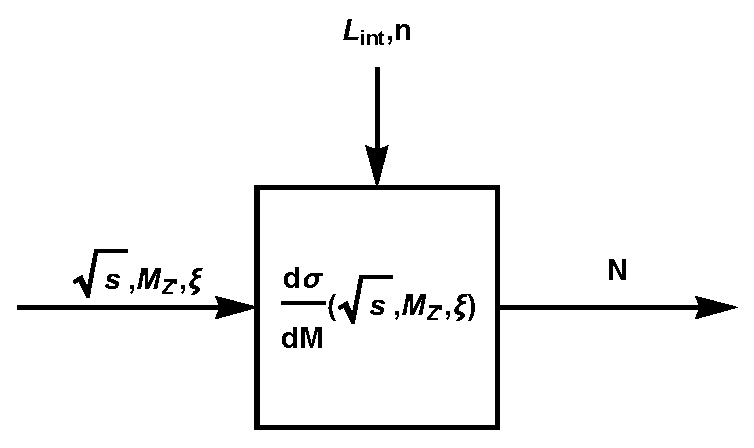
\includegraphics[width=0.5\textwidth]{figures/model.eps}
	\caption{Схема объекта исследования при построении экспериментальной
		факторной модели}
	\label{fig:schema-model}
\end{figure}

Входными переменными являются $\sqrt{s}$ -- энергия протона, ${M}_{{Z}^{\prime}}$ -- масса $Z'$ бозона, $\xi$ -- угол смешивания, ${L}_{int}$ -- светимость установки, $n$ -- количество генерируемых событий. Выходным значением является количество событий в сечении $N$ для заданной ширины ${M}_{{Z}^{\prime}}$.

При построении экспериментальной факторной модели объект
моделирования (проектируемая техническая система) представляется в виде
«черного ящика», на вход которого подаются некоторые переменные, a на
выходе можно наблюдать и регистрировать переменные. 

Они являются внутренними и внешними параметрами объекта проектирования,
подлежащие оптимизации, а выходными переменными <<черного ящика>>
являются выходные параметры объекта, характеризующие его эффективность и
качество процессов функционирования, выбираемые в качестве критериев
оптимальности. В процессе проведения эксперимента изменение входных
переменных приводит к изменениям выходных переменных. Для построения
факторной модели были зарегистрированы эти изменения и осуществлена
необходимая статистическая обработка для определения параметров модели.
\section{Выводы}
В результате проведенных исследований была разработана
математическая модель для моделирования процесса рождения ${Z}^{\prime}$-бозонов в протон-протнных столкновениях с учетом эффектов $Z$-${Z}^{\prime}$ смешивания в условиях выполненных экспериментов на \textit{ATLAS}, а также
возможностью задания входных параметров.


\chapter{РАЗРАБОТКА ИМИТАЦИОННОЙ МОДЕЛИ И СРЕДСТВ РЕАЛИЗАЦИИ ИМИТАЦИОННОГО МОДЕЛИРОВАНИЯ}
\section{Процесс рождения $Z^\prime$-бозонов в протон-протонных столкновениях с учетом эффектов $Z$-$Z^\prime$ смешивания}
Многие сценарии Новой Физики (НФ) отличной от Стандратной Модели (СМ)~\cite{2part-1}, включая модель суперпозиций и левую-правую симметричную модель, предсказывают существование новых нейтральных и заряженных калибровочных бозонов, которые могут быть найдены на текущих или будущих коллайдерах. Поиск нового нейтрального $Z^\prime$ и заряженного $W^\prime$ калибровочных бозонов является важным аспектом экспереметально-физических программ на колладерах больших энергий. В этой работе сконцентрировано внимание на первом бозоне.

Предоставленные лимиты большого адронного коллайдера и виртуальные эффекты ЛЭП, через интерференцию или смешивания с $Z$ бозонами, подразумевает что любые $Z^\prime$ бозоны горазда тяжелее и менее смешиваются с $Z$ бозонами. В зависимости от рассматриваемой теоретической модели $Z$ массы порядка 4,5 ТэВ~\cite{2part-pankov} и $Z-Z^\prime$ углов смешивания на уровне нескольких градусов исключены~\cite{sirunyan:2017}. Угол смешивания сильно ограничен очень высокоточными экспериментами на ЛЭП и \textit{SLC}. Они включают в себя измерения из формы линии \textit{Z}, из лептонных отношений ветвления, нормированных на общую адронную ширину затухания $Z$, а также от лептонных лево-правых асимметрий. $Z^\prime$, легче чем 5 ТэВ, может быть обнаружен на БАК~\cite{sirunyan:2017} c $\sqrt{s} = 14 $ ТэВ в процессе Дрелл-Янга (ДЯ) $pp \rightarrow Z^\prime \rightarrow l^+l^- + X$, где $l=e,\mu$.

После открытия $Z^\prime$-бозона на БАК через процесс ДЯ, необходимо произвести некоторую диагностику связей и смешивания $Z$-$Z^\prime$, чтобы идентифицировать основную теоретическую структуру. В настоящей работе исследуются данные \textit{ATLAS}~\cite{main-book} и \textit{CMS} в канале дибозона:

\begin{equation} \label{eq:1}
pp \rightarrow W^+W^- + X.
\end{equation}

Для поиска \textit{Z}-бозона, который возникает, например, в популярной модели с расширенным калибровочным сектором~\ref{eq:1}. Анализ основан на данных о столкновениях $pp$ при энергии центра масс $\sqrt{s} = 13 $ собранных группами \textit{ATLAS}~\cite{main-book} и \textit{CMS} на БАК. В частности, данные используются для поиска $Z$-$Z^\prime$ смешивание. На \textit{ATLAS} события $W^+W^-$ реконструируются через их полулептонные распады $W$, где один $W$-бозон распадается на заряженный лептон ($l=e,\mu$) и нейтрино, а другой на две струи, тогда как на CMS $W$-бозон адронически распадается на две восстановленные струи. 

Процесс рождения пары $W^-W^+$-бозонов~\ref{eq:1} важен для изучения электрослабой калибровочной симметрии. Общие свойства слабых калибровочных бозонов тесно связаны с нарушением электрослабой симметрии и структуры калибровочного сектора, как и существование и структура трилинейных связей. Кроме того, канал распада дибозонов $Z^\prime$ исследует толщину калибровочной связи между новым и калибровочными бозонами стандартной модели. Кроме того, сила связи очень влияет на элементы распада и естественную ширину такого нового калибровочного бозона. Таким образом, детальное рассмотрение процесса~\ref{eq:1} с высокой точностью проверяет калибровочный сектор СM и может пролить свет на бозоны, которые могут появиться за пределами СМ. Здесь мы рассмотрим возможность наблюдения $Z^\prime$-бозона в $W^+W^-$ парного процесса на БАК, который в отличие от процесса ДЯ не является основным каналом поиска, но может помочь понять происхождение новых калибровочных бозонов.

Поиски тяжелого \textit{WW} резонанса были выполнены на Теватроне исследовательскими группами \textit{CDF} и \textit{D0}. Группа \textit{D0} изучала резонансное рождение дибозонов до 700 ГэВ в каналах распада $lvl^\prime v^\prime$ и $lvjj$~\cite{Krasnikov:2004}. Группа \textit{CDF} также исследовала резонанс в $WW$ в канале распада $evjj$, что в результате привело к обнаружения нижних лимитов масс $Z^\prime$
и $W^\prime$-бозонов, за исключением масс превышающих 900 ГэВ, зависящих от параметра смешивания.

Исследования \textit{WW}-резонансов группами \textit{ATLAS} и \textit{CMS} с использованием, соответственно, полулептонных и адронных событий распада в $pp$ столкновениях при 13 ТэВ устанавливают массовые пределы 3 ТэВ для этих резонансов~\cite{nuclphys:weak}. 

В диссертационной работе изучается возможность рождения нового резонанса нейтрального спина 1 ($Z^\prime$) из доступных данных групп \textit{ATLAS} для $W^+W^-$ распадов. В качестве результатов работы будут получены ограничения на соответствующие $Z-Z^\prime$-коэффициенты смешивания и на массу $M_{Z^\prime}$.
Выполнено моделирование событий рождения $Z^\prime$ бозонов в процессе распада на фотонную пару и моделирование событий рождения гравитонов в процессе $lvl^\prime v^\prime$. Создано \textit{web}-приложение для демонстрации результатов вычисления.

Несмотря на впечатляющий успех в описании экспериментов, Стандартная модель не может считаться окончательной теорией элементарных частиц. У нее есть свои трудности. Физики уверены, что она должна быть частью некоторой более глубокой теории строения микромира, той частью, которая видна в экспериментах на коллайдерах при энергиях ниже примерно 1 ТэВ. Главная задача Большого адронного коллайдера — получить хотя бы первые намеки на то, что это за более глубокая теория.

Теоретики разработали большое число кандидатов на такую теорию. Все они, естественно, включают какие-то элементы, которые отсутствуют в Стандартной модели. Часто такие теории коллективно называют «Новая физика» или «За пределами Стандартной модели». На этой странице перечислены некоторые из активно изучаемых вариантов Новой физики~\cite{2part-1}.

\begin{figure}[h]
	\centering
	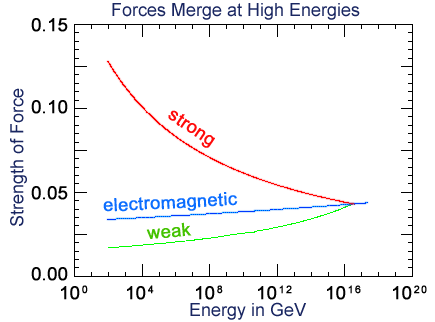
\includegraphics[width=\textwidth]{figures/hep-sm.png}
	\caption{Константы связи трех типов взаимодействий}
	\label{fig:fig01}
\end{figure}

Суперсимметрия -- это гипотетическая симметрия между фермионами и бозонами. Теории, использующие эту идею, оказываются удивительно мощными, и потому именно с суперсимметрией многие связывают надежды на открытие физики за пределами Стандартной модели. Однако до сих пор не было получено ни одного убедительного доказательства в пользу того, что суперсимметрия реализуется в нашем мире. Ее поиск является одной из главных задач Большого адронного коллайдера.

Константы связи трех взаимодействий частиц в микромире сходятся к одному значению, если имеющиеся сейчас данные экстраполировать в область очень высоких энергий. Это совпадение считается неслучайным и воспринимается физиками как намек на то, что все три взаимодействия при больших энергиях объединяются в одно.

В XIX веке физики обнаружили, что электричество и магнетизм — это две стороны одной медали, электромагнитного взаимодействия. Век спустя, при создании Стандартной модели, электромагнетизм и слабые ядерные силы были объединены в рамках единого электрослабого взаимодействия. Точнее говоря, внутри электрослабого взаимодействия имеются по-прежнему две разные силы, а электромагнитное и слабое взаимодействия возникают как комбинации этих сил. Каждое такое объединение упрощало теорию, уменьшало количество введенных в нее «сущностей», переводило наше понимание микромира на новый уровень.

Сейчас физики имеют сразу несколько причин подозревать, что при очень высоких энергиях происходит объединение электрослабого и сильного взаимодействий (рисунок~\ref{fig:fig01}). Модели, использующие эту идею (так называемые Теории великого объединения) разрабатываются уже давно. В идеале хотелось бы, чтобы такая теория естественным образом объясняла, почему фундаментальных взаимодействий именно столько и именно с такими свойствами, а также имела четкие предсказания, доступные проверке в современных экспериментах~\cite{main-book2}.

При энергиях элементарных частиц, доступных на ускорителях, гравитация по-прежнему остается исключительно слабой, так что заметить ее проявления не удается. Однако ее сила растет с ростом энергии, и при энергиях столкновения порядка планковской она станет столь же важной, как и другие взаимодействия. В этом случае в полный рост встает исключительно сложный вопрос о том, как включить гравитацию в квантовое описание микромира. Поскольку гравитация в современной физике считается проявлением кривизны пространства-времени, успешная теория с сильной гравитацией должна описывать в рамках единого формализма не только все взаимодействия и всё вещество, но и структуру пространства-времени.

Одним из наиболее привлекательных путей решения этого вопроса является теория суперструн и ее дальнейшее развитие в виде теории бран и М-теории. В этих теориях считается, что фундаментальными объектами, существующими в многомерной вселенной, являются не точечные частицы, а протяженные объекты -- струны, мембраны и еще более многомерные образования. В этой теории были получены впечатляющие успехи при высоких энергиях, однако при попытке вывести свойства нашего низкоэнергетического мира из теории суперструн возникает обескураживающая неопределенность предсказаний.

Долгое время казалось, что проверка предсказаний теории суперструн лежит далеко за пределами возможностей человечества, поскольку речь идет об энергиях, на 15 порядков превышающих энергии современных ускорителей. Однако примерно 10 лет назад возникло новое направление развития теории, в котором гравитация становится сильной на энергиях порядка 1 ТэВ. Такая возможность возникает в том случае, если наш мир более чем трехмерный и если при этом новые дополнительные пространственные размерности достаточно протяженны: либо они бесконечны, либо свернуты в многомерные петельки размером много больше ядерного масштаба.

В этом случае на \textit{LHC} следует ожидать целый ряд совершенно замечательных эффектов, отсутствующих в Стандартной модели, например, рождение гравитонов, которые будут улетать из нашего мира в дополнительные измерения, и микроскопических черных дыр, тут же испаряющихся с испусканием множества обычных частиц. Будут также наблюдаться сильные отклонения от предсказаний Стандартной модели в столкновении обычных частиц. Стоит, впрочем, подчеркнуть, что пока нет никаких экспериментальных подтверждений того, что эта красивая гипотеза имеет отношение к нашему миру.

Все три перечисленные выше направления «Новой физики» опираются на глубокие теоретические гипотезы об устройстве нашего мира (суперсимметрия, единство сил, квантово-гравитационная вселенная). Однако кроме этих направлений теоретики также рассматривают разнообразные теории «статусом пониже». В этих теориях просто отмечается, что текущие экспериментальные данные не запрещают те или иные экзотические объекты или явления, и разрабатываются их следствия. Вот несколько примеров таких моделей разной степени экзотичности.

Неминимальные хиггсовские модели. Поскольку хиггсовские бозоны — единственные частицы Стандартной модели, до сих пор не открытые экспериментально, теоретики изучают самые разные варианты устройства этого сектора теории.
Новые поколения фермионов. Можно предположить, что кроме трех известных поколений кварков и лептонов существуют и другие поколения. Частицы из этих поколений должны быть очень тяжелыми, иначе бы их уже давно открыли в эксперименте.

Новые короткодействующие силы. В таких моделях предполагается, что в нашем мире есть и иные силовые взаимодействия, отличные от сильных, слабых и электромагнитных, но они настолько короткодействующие, что до сих пор никак не проявлялись в эксперименте. На Большом адронном коллайдере благодаря его рекордной энергии удается «прощупать» взаимодействия частиц на исключительно малых расстояниях (менее 10–19 метра), а значит, появляется шанс эти взаимодействия обнаружить. Они могут проявляться либо как рождение и распад частицы-переносчика новых сил (такие гипотетические частицы обозначают $Z^\prime$), либо как усиленное рассеяние частиц на большие углы.

\begin{figure}[h]
	\centering
	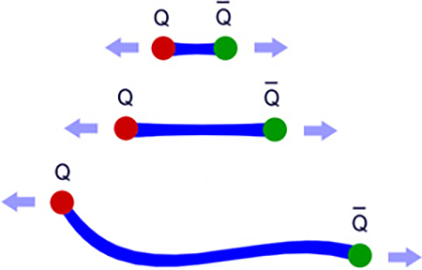
\includegraphics[width=\textwidth]{figures/quirk-antiquirk.jpg}
	\caption{Кварки}
	\label{fig:fig03}
\end{figure}

Лептокварки. В Стандартной модели и в подавляющем большинстве теорий Новой физики кварки и лептоны взаимодействуют друг с другом опосредованно, путем обмена квантами силовых полей. Однако можно представить себе возможность того, что кварки и лептоны исходно являлись фермионами одного типа и лишь потом расщепились на два разных сорта. В таком случае должны существовать новые тяжелые частицы — лептокварки, которые распадаются прямо на кварк и лептон. Подобные частицы встречаются в теориях Великого объединения.

Квирки. Одним из очень необычных и любопытных вариантов новых сил является гипотеза квирков (\textit{quirks}). Эта модель построена по типу обычного сильного взаимодействия: в ней предполагается, что существует новое силовое поле с конфайнментом и новые частицы, его чувствующие. Если частицы очень тяжелые, то между ними будут натягиваться длинные, даже макроскопические силовые струны, которые не смогут порваться (рисунок~\ref{fig:fig03}).

Слабое взаимодействие – короткодействующее фундаментальное взаимодействие между элементарными частицами, ответственное за бета-распад атомных ядер и медленные распады частиц. Слабое взаимодействие значительно слабее сильного и электромагнитного, но гораздо сильнее гравитационного. В слабом взаимодействии участвуют все фундаментальные фермионы (кварки и лептоны) и все адроны. Единственными частицами, которые участвуют только в слабом взаимодействии являются три типа нейтрино $v_e$, $v_\mu$, $v_\tau$ и их античастицы  антинейтрино $\bar{v_e}$,  антинейтрино $\bar{v_\mu}$,  антинейтрино $\bar{v_\tau}$. В нем не участвуют переносчики сильного, электромагнитного и гравитационного взаимодействий -- глюон, фотон и гравитон. В процессе слабого взаимодействия частицы обмениваются переносчиками слабого взаимодействия промежуточными (фундаментальными) бозонами: имеющими электрический заряд $W^±$ и нейтральным $Z$. Эти бозоны, в отличие от переносчиков остальных фундаментальных сил безмассовых глюона, фотона и гравитона, имеют огромные массы $m_W$ = 80.4 ГэВ/с~${}^2$ и $m_Z$ = 91.2 ГэВ/с${}^2$ (примерно как у атомов циркония или ниобия), что приводит к очень малому радиусу действия слабых сил ≈10-18 см (что на три порядка меньше радиуса сильного взаимодействия) и очень низкой по сравнению с сильными и электромагнитными процессами вероятности (скорости) слабых процессов.

Несмотря на малую величину и короткодействие слабые силы играют очень важную роль в природе. Так без них погасло бы Солнце, так как внутри него остановился бы процесс превращения 4 протонов в ядро гелия-4, являющийся основным источником энергии Солнца.

Слабое взаимодействие выделяется тем, что в нём не соблюдается ряд запретов, присущих сильному и электромагнитному взаимодействиям. Так в слабых процессах кварки одного типа (аромата) превращаются в кварки других ароматов~\cite{nuclphys:weak}.

Особенности слабого взаимодействия:
\begin{enumerate}
	\item[--] их слабость (медленность), выражающаяся в том, что
	вероятность этих процессов на много порядков меньше
	вероятностей сильных и электромагнитных процессов;
	
	\item[--] малый радиус взаимодействия —как минимум на
	два порядка меньший, чем радиус сильного взаимодействия.
	Ни в одном из слабых процессов не удалось до 1982 г. обнаружить каких-либо отклонений от точечного четырех-
	фермионного взаимодействия;
	
	\item[--] сильное, максимально возможное несохранение пространственной и зарядовой четностей. Так, в заряженные
	токи входят только левые компоненты спиноров, описывающих частицы, и только правые компоненты спиноров,
	описывающих античастицы;
	
	\item[--] несохранение \textit{СР}-четности;
	
	\item[--] несохранение ароматов (странности, чарма и т. д.);
	
	\item[--]  то обстоятельство, что только в слабых взаимодействиях принимают участие нейтрино.
	
\end{enumerate}

Тем поразительней, что, несмотря на столь резкие отличия, слабые и электромагнитные взаимодействия представляют собой, по-видимому, проявление одного и того же
взаимодействия, которое в последние годы получило название электрослабого.

Согласно электрослабой теории слабые взаимодействия
заряженных токов обусловлены обменами $W$-бозонами, а
нейтральных -- $Z$-бозонами, подобно тому как взаимодействие электромагнитных токов обусловлено обменом фотонами. При этом слабость и малый радиус слабого взаимодействия объясняются тем, что, в отличие от фотонов, $W$ и $Z$-бозоны -- очень тяжелые частицы Остальные особенности слабого взаимодействия прямо заложены в предположении о форме исходных фермионных токов теории.
Так что в злектрослабой теории удивляться надо не тому,
что слабое взаимодействие зеркально-асимметрично, a тому, что электромагнитное -- зеркально-симметричное.

Слабое взаимодействие переносится массивными $W^±$- и $Z$-бозонами. Обмен заряженными $W^+$ и $W^-$-бозонами приводит к изменению электрического заряда взаимодействующих фермионов. Эти процессы происходят за счет заряженных токов.





В физических программаx экспериментов на  современных  дронных (\textit{LHC}) и планируемых на  электрон-позитронных (\textit{ILC, CLIC}) коллайдерах вопросу поиск  <<новой>> физики, выходящей за  рамки Стандартной модели (СМ), традиционно уделяется большое внимание. К числу подобных теоретических построений, являющихся обобщением СМ, относятся модели с расширенным к либровочным сектором, такие как лево-правосимметричные модели (\textit{LR}), альтернативные лево-правосимметричные модели (\textit{ALR}), $E_6$-модели
и др.~\cite{Bobovnikov:2016}. Их исследование (теоретическое и экспериментальное) представляет значительный интерес. Эти модели являются одними из простейших расширений СМ, характеризующихся элементарной структурой хиггсовского сектора. Общим для данных моделей является то, что они предсказывают новые физические объекты и явления на масштабе энергий $O$ (1 ТэВ), связанные, например, с наличием тяжелых нейтральных ($Z^\prime$) калибровочных бозонов, обусловленных дополнительными калибровочными симметриями $U(1)^\prime$.

Достижение порога рождения $Z^\prime$-бозона явилось бы прямым доказательством проявления «новой» физики. Однако в данном случае интервал поиска масс $Z^\prime$ ограничен максимальной энергией коллайдера, на котором проводятся эксперименты. Значительно более широкий интервал масс можно исследовать с помощью пропагаторных эффектов. В этом случае ведется поиск отклонений различных наблюдаемых от соответствующих предсказаний СМ. Если экспериментальные данные при достигнутом уровне точности согласуются с СМ, т. е. отклонений от предсказаний СМ нет, то эту экспериментальную информацию можно использовать для получения ограничений на динамические параметры и массы $Z^\prime$-бозонов.

Потенциальные возможности $e^+$$e^-$-коллайдеров для прямого рождения новых калибровочных бозонов гораздо скромнее по сравнению с адронными машинами из-за более низких энергий пучков. Кроме того, современные ограничения на массы $Z^\prime$-бозонов для большинства моделей превосходят планируемую энергию электрон-позитронного коллайдера \textit{ILC}, $\sqrt{s}<< M_{Z^\prime}$. Тем не менее основным достоинством этих машин является возможность проведения экспериментов по измерению наблюдаемых величин с высокой степенью точности и получения однозначной информации о косвенных (виртуальных) эффектах новых $Z^\prime$-бозонов, а также эффектах бозонного $Z$-$Z^\prime$-смешивания. Последние, в моделях с расширенным калибровочным сектором, зависят от структуры хиггсовского сектора модели. Тем самым экспериментальное исследование процессов рождения пар $W^±$-бозонов может не только пролить свет на возможное существование <<новой>> физики, но и дать косвенные указания на хиггсовскую природу, а также установить структуру модели.

На основе данных, полученных из низкоэнергетических экспериментов по нейтральным токам, результатов на $e^+e^-$-коллайдерах \textit{LEP} и \textit{SLC}~\cite{Bobovnikov:2016}, а также недавно выполненных экспериментов по поиску прямого адронного рождения $Z^\prime$-бозонов в процессе Дрелла-Яна:
\begin{equation} \label{eq:drell}
	pp \rightarrow Z^\prime \rightarrow l^+l^- + X
\end{equation}
где $l=e,\mu$) на коллайдере \textit{LНC} при энергии $\sqrt{s}$ = 7 и 8 ТэВ с интегральной светимостью соответственно $L_int$ = 5 и 20 фб${}^{-1}$~\cite{Bobovnikov:2016} можно заключить, что для большинства расширенных калибровочных моделей граничные значения для масс дополнительных $Z^\prime$- бозонов находятся в интервале $\sim$ 2,5-3,0 ТэВ (в зависимости от модели), а современный масштаб ограничений на угол смешивания составляет $\mathcal{O}(\varphi )$ ~ ${10}^{-2}$--${10}^{-3}$ рад. При этом наиболее точная информация об угле смешивания была получена преимущественно из экспериментов на электрон-позитронных коллайдерах \textit{LEP1}~\cite{schael:2006} и \textit{SLC} по измерению резонансных наблюдаемых физических величин при энергии начальных состояний, равной массе стандартного $Z$-бозона, $\sqrt{s}$ = $M_Z$, в процессах:
\begin{equation} \label{eq:drell2}
	e^+e^- \rightarrow f\bar{f}
\end{equation}
где конечными фермионными состояниями $f$ были заряженные лептоны и кварки~\cite{andreev-pankov:2012}. Высокая точность, достигнутая в экспериментах на коллайдерах \textit{LEP1} и \textit{SLC}, объясняется прежде всего возможностью набора большого объема данных в резонансной области энергии.

Кроме того, эта информация дополнялась данными, полученными на коллайдере тэватрон, по точному измерению массы $M_W$, на основе которых определялся параметр бозонного $Z$−$Z^\prime$-смешивания с использованием соотношения между массами нейтральных и заряженных калибровочных бозонов, $M_Z$ = $M_W$/$(\sqrt{p_0}\cos\theta_W)$, имеющего место в расширенных моделях. Очевидно также, что эти данные будут дополнены новой информацией, которая в ближайшем будущем будет получена в экспериментах на коллайдере \textit{LНС} при энергии 13 и 14 ТэВ. Вместе с тем из этих данных нельзя сделать однозначный вывод о природе «новой» физики, который мог бы вызвать отклонение наблюдаемых величин от их поведения, предсказываемого СМ. Дело в том, что параметр $p$, который содержится в выражениях для векторных и аксиально-векторных констант связи фермионов с учетом петлевых поправок, зависит, в частности, от структуры хиггсовского сектора модели, которая изначально неизвестна. Кроме того, новые тяжелые фермионы и скалярные частицы, предсказываемые моделями с расширенным калибровочным сектором, могут давать вклад в параметр $p$ на петлевом уровне. Все эти неопределенности приводят к появлению систематических (теоретических) погрешностей, которые могут быть весьма существенными при измерении параметра $p$ и, в конечном счете, могут повлиять на точность определения параметра $Z$−$Z^\prime$-смешивания.

Процессы парного рождения заряженных $W^±$-бозонов в адронных столкновениях на \textit{LНС}:
\begin{equation} \label{eq:drell3}
	pp \rightarrow W^+W^- + X
\end{equation}

Процессы электрон-позитронной аннигиляции на \textit{LЕР2} и в большей степени на \textit{ILС}:
\begin{equation} \label{eq:drell4}
	e^+e^- \rightarrow W^+W^-
\end{equation}

Являются весьма эффективным инструментом поиска эффектов $Z$−$Z^\prime$-смешивания при высоких энергиях и, таким образом, играют роль основного поставщика информации об угле $Z$−$Z^\prime$-смешивания~\cite{Bobovnikov:2016}. С теоретической точки зрения процессы парного рождения заряженных калибровочных бозонов в адронных и электронпозитронных столкновениях интересны тем, что их сечения пропорциональны углу $Z$−$Z^\prime$-смешивания, который, как отмечалось выше, в расширенных калибровочных моделях зависит от структуры сектора Хиггса~\cite{sirunyan:2017}.

Прямой поиск тяжелых резонансов в процессе $p\bar{p} \rightarrow W^+W^- + X$ осуществлялся экспериментальными группами \textit{СDF} и \textit{D0} на коллайдере тэватрон. Коллаборация \textit{D0} исследовала возможность рождения резонанса в канале его дибозонного распада, используя чисто лептонные $lvl^\prime v^\prime$ и полулептонные $vjj$ моды. Здесь $l=e,\mu$; $jj$ — две адронные струи. Коллаборация \textit{СDF} также осуществляла поиск тяжелых резонансов в канале их распада в пару заряженных калибровочных бозонов $W^+W^−$ с последующим распадом в полулептонные $evjj$ конечные состояния. Обе коллаборации установили ограничения на массы тяжелых резонансов, таких как новые нейтральные $Z^\prime$- и заряженные калибровочные $W^±$-бозоны, гравитоны Рэндалл-Сандрума. Кроме того, в настоящее время поиск тяжелых резонансов на \textit{LHC} в \textit{WW}-канале интенсивно ведется коллаборациями \textit{ATLAS} и \textit{CMS}. В частности, уже получена экспериментальная информация о процессе в лептонном канале $lvl^\prime v^\prime$ при энергии коллайдера 7 ТэВ и интегральной светимости 4,7 фб${}^{−1}$~\cite{2part-pankov}.

Из анализа экспериментальных данных по измерению процесса электрон-позитронной аннигиляции на коллайдере \textit{LEP2} были впервые получены прямые ограничения на угол $Z$−$Z^\prime$-смешивания. Точность измерения угла смешивания оказалась не очень высокой, $\left |\phi \right |$~5—10 \%, так как сам коллайдер работал в интервале энергий, незначительно превышающем порог реакции, $\sqrt{s} >> 2M_W$. Как было установлено ранее, чувствительность процесса электрон-позитронной аннигиляции к эффектам «новой» физики значительно усиливается при высоких энергиях, $\sqrt{s} >> 2M_W$, где важную роль играет механизм калибровочного сокращения. Дело в том, что вклад $Z^\prime$-бозона в сечение процесса нарушает механизм калибровочного сокращения, играющий важную роль в СМ~\cite{andreev-ee:2012}. Действие механизма калибровочного сокращения состоит в том, что он обеспечивает «правильное» поведение сечения процесса электрон-позитронной аннигиляции с ростом энергии, которое не нарушает унитарный предел, несмотря на быстро растущие с энергией отдельные вклады в сечение. Вместе с тем эффекты, индуцированные появлением дополнительного калибровочного бозона, нарушают механизм калибровочного сокращения в энергетическом интервале $2M_W << \sqrt{s} << M_{Z^\prime}$, что проявляется в виде «разбалансировки» отдельных вкладов в сечение и, как следствие, в возникновении существенно иной по сравнению со СМ энергетической зависимостью сечений. Этим обусловлено действие так называемого механизма усиления эффектов «новой» физики в процессе электрон-позитронной аннигиляции. Именно в силу этого обстоятельства линейный коллайдер \textit{ILC} является одним из основных инструментариев для поиска эффектов «новой» физики при исследовании процесса электрон-позитронной аннигиляции.

Следует отметить также, что коллаборация \textit{CDF} на коллайдере тэватрон одной из первых получила прямые ограничения на угол $Z$−$Z^\prime$-смешивания из обработки данных по измерению процесса адронного рождения $W^+W^−$-бозонов. И вновь относительно небольшая энергия установки и низкая светимость не позволили улучшить ограничения, полученные на коллайдере \textit{LEP2}, а лишь повторить их~\cite{ada-wwz:2013}.

Возможности коллайдера \textit{LНС} по обнаружению эффектов $Z$−$Z^\prime$-смешивания в процессе рождения пар заряженных калибровочных $W^±$-бозонов с их последующим распадом по чисто лептонному каналу $lvl^\prime v^\prime$. Несмотря на очевидное достоинство данного канала, связанное с подавленностью фона, особенно при больших инвариантных массах $W^±$-бозонов, у него имеется заметный недостаток, связанный с присутствием в конечных фермионных состояниях двух нейтрино, что не позволяет восстановить распределение по инвариантной массе бозонных пар из экспериментальных данных. В то же время распад пары $W^±$-бозонов по полулептонному каналу $lvjj$ свободен от указанного недостатка. В процессе $pp \rightarrow Z^\prime \rightarrow WW + X \rightarrow lvjj + X$ существует возможность реконструировать распределение по инвариантной массе $W^+W^-$- пары и тем самым исследовать резонансную структуру $Z^\prime$-бозона. Еще одним достоинством настоящего полулептонного процесса является то, что он имеет сечение, существенно превосходящее сечение чисто лептонного канала. Вместе с тем полулептонный канал, в отличие от лептонного канала $lvl^\prime v^\prime$, имеет большой КХД-фон, вызванный рождением $W_{jj}$-, а также $Z_{jj}$-состояний~\cite{ada-lvlv:2013}. В последнем случае предполагается, что $Z$-бозон распадается по лептонному каналу, а в процессе детектирования лептонов один из них теряется. Кроме перечисленных выше КХД фоновых процессов имеется еще один, который играет важную роль в оценке всей фоновой составляющей. Это процесс рождения пар $t\bar{t}$-кварков. Однако большой КХД-фон может быть редуцирован путем наложения кинематических ограничений на поперечные импульсы заряженных лептонов и адронных струй в резонансном сигнале рождения $Z^\prime$-бозонов~\cite{Bobovnikov:2016}.


\section{Описание блок-схемы программного комплекса
	моделирования}
Блок-схема разработанного программного комплекса имитационного
моделирования представлена на рисунке~\ref{fig:ui-block-schema}.

\begin{figure}[!h]
	\centering
	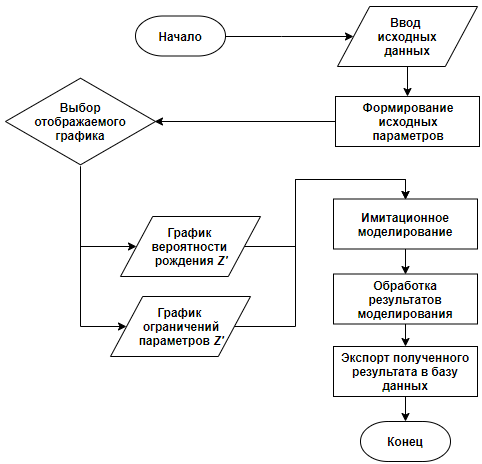
\includegraphics[width=\textwidth]{figures/ui-schema.png}
	\caption{Блок-схема программного комплекса имитационного моделирования}
	\label{fig:ui-block-schema}
\end{figure}

После открытия интерфейса приложения происходит начальная инициализация
(программный код представлен в приложении А), которая не видна
пользователю. Затем открывается главное окно интерфейса программного
комплекса.

Затем происходит формирование исходных параметров и пользователю
необходимо выбрать какой график необходимо вывести на экран. 

Если же
график не выбран, то будет выведена веб страница с описанием программного комплекса. После выбора Графика происходит имитационное моделирование по заданным параметрам. Далее
происходит обработка результатов моделирования и экспорт полученного
результата в базу данных, что позволяет не потерять накопленный результат и не затрачивать ресурсы на повторное моделирование. В качестве базы данных используется нереляционная база данных \textit{Redis}, отличающаяся от реляционных баз данных быстрым способом чтения и записи данных в виде ключ-значение. Так же используется сервис \textit{AWS ElastiCache}  разработанный компанией \textit{Amazon}, что позволяет огранизовать общий доступ для исследователей к результатам моделирования.
\section{Разработка программы и средств реализации имитационного моделирования}
В наши дни, когда компьютерные технологии бурно развиваются, не
всегда удается создать сложное приложение, используя один язык
программирования. Разные языки имеют свои преимущества и недостатки и как
правило, что ни один из них не удовлетворят требованиям разрабатываемой
прикладной программы. Выходом из такого положения является использование
нескольких языков программирования. Такой подход часто используется при
создании программ для научных исследований, управления производственными
процессами и других коммерческих приложений. При этом приходится решать
задачи взаимодействия компонентов, написанных, которые написаны на на
разных языках программирования. Компоненты, реализующие графический
интерфейс пользователя, управление базами данных, получение и обработку
данных в реальном времени, как правило интегрируются в одно приложение.

Для реализации поставленной задачи исследования в магистерской
диссертации был выбран пакет моделирования процессов столкновения элементарных частиц при высоких энергиях на ускорителях элементарных частиц \textit{PYTHIA} на языке программирования \textit{С++}, а также принято решение о реализации всего программного
комплекса на языке программирования \textit{Java}.
В качестве веб интерфейса был использован фреймворк \textit{Angular} на языке программирования \textit{JavaScript}. Так же была использована и бибилотека \textit{d3js} для отрисовки графиков в виде \textit{SVG} изображений и взаимодейсвия пользователся с интерфейсом приложения.

Когда говорят о научных основах проектирования пользовательских
интерфейсов, в первую очередь упоминают термин \textit{Human-Computer Interaction}
(\textit{HCI}) – «взаимодействие человека и компьютера». В странах Запада \textit{HCI} это
является целой профессией, ей обучают в университетах, издается много
журналов по этой теме, существует большое количество Web-сайтов.
Составными частями \textit{HCI} являются:

\begin{enumerate}
	\item[--] человек (пользователь);
	\item[--] компьютер;
	\item[--] их взаимодействие.
\end{enumerate}

Пользовательский интерфейс \textit{user interface} (\textit{UI}) – является своеобразным
коммуникационным каналом, по которому осуществляется взаимодействие
пользователя и компьютера.

Лучший пользовательский интерфейс – это такой интерфейс, которому
пользователь не должен уделять много внимания, почти не замечать его. В руках
пользователя интерфейс пользователя должен служить инструментом для
достижения цели. Такой интерфейс называют прозрачным – пользователь
смотрит сквозь него на свою работу.

Чтобы создать эффективный интерфейс, который делал бы работу с
программным комплексом эффективной, нужно понимать, какие задачи будут
решать пользователи с помощью данной программного комплекса и какие
требования к интерфейсу могут возникнуть у пользователей. Большую роль в
разработке интерфейса играет интуиция – если разработчик сам терпеть не
может некрасивые и неудобные интерфейсы, то при создании собственного
программного комплекса он будет чувствовать, где и какой именно элемент
нужно убрать или добавить. Необходимо иметь художественный вкус, чтобы
понимать, что именно придаст интерфейсу красоту и привлекательность.

Западные исследователи в области \textit{HCI} сформулировали основные
принципы проектирования пользовательских интерфейсов компьютерных
программ~\cite{user-interface}. Как и в любой другой отрасли ИТ, существует довольно много
различных методик и классификаций. Можно сформировать три положения
говоря об общих принципах проектирования пользовательского интерфейса:

\begin{enumerate}
	\item[--] программный комплекс должен помогать выполнить задачу, а не
	становиться этой задачей;
	\item[--] при работе с программой пользователь не должен думать, что он не
	понимает программу;

	\item[--] программный комплекс должен работать так, чтобы пользователь не
	считал компьютер бесполезным инструментом.
\end{enumerate}

Конечно, глубина проработки интерфейса и степень его адаптивности под
нужды пользователя в программных комплексах в основном зависит от усилий
их авторов, а не от характеристик аппаратного обеспечения. Однако у
большинства пользователей компьютер ассоциируется именно с программными
комплексами, которые на нем работают, и плохое впечатление от использования
программного обеспечения автоматически переносится на сам компьютер.

Сообщество разработчиков фреймворка \textit{Angular} разрабатывает дополнительные компоненты \textit{Angular Material Design} и предлагает использовать их для быстой разработки приложения с нуля. 

\textit{Material Design} -- визуальный язык, представлен в 2014 году \textit{Google}, используется чаще всего в мобильных приложения. Пример использования \textit{Material Design} можно увидеть во многих мобильных приложения Google(Play, Music, Books и т.д.), а также в Chrome OS. Material Design упрощает разработчикам настройку UI, сохраняя при этом удобный интерфейс приложений. Angular Material состоит из набора предустановленных компонентов Angular. Anglate Material стремится обеспечить расширенный и последовательный пользовательский интерфейс. В то же время он дает возможность контролировать, как ведут себя разные компоненты.

Открыв начальную веб-страницу приложения в любом из доступных браузеров пользователь увидит сообщение с описанием проекта, как показано на рисунке~\ref{fig:welcome-page}.

\vspace{16pt}
\begin{figure}[!h]
	\centering
	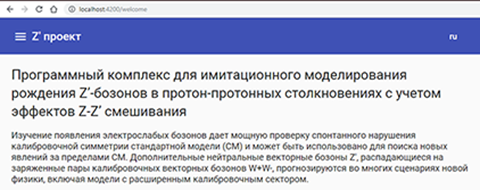
\includegraphics[width=\textwidth]{figures/welcome-page.png}
	\caption{Начальная \textit{web}-страница}
	\label{fig:welcome-page}
\end{figure}

Для каждого пользователя на начально странице приложения распологается навигационное меню, котрое показано на рисунке~\ref{fig:menu}. Так как разработанное приложение является одностраничным то переход по пунктам меню не перезагружает страницу полностью, а лишь догружает необходимые компоненты.

\begin{figure}[!h]
	\centering
	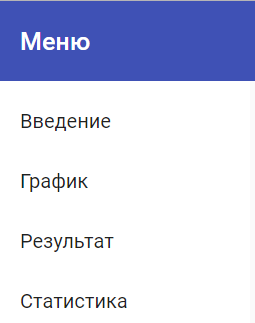
\includegraphics[width=0.5\textwidth]{figures/menu.png}
	\caption{Главное меню приложения}
	\label{fig:menu}
\end{figure}
\vspace{5cm}
Из главного меню доступен переход на следующие страницы приложения: 

\begin{enumerate}
	\item[--] <<Введение>> -- начальная страница \textit{web}-приложения;
	\item[--] <<График>> -- страницы с основным графиком и панелью для ввода параметров и отравки запроса на вычисление;
	\item[--] <<Результат>> -- страница предосталяющая полученные результаты на угол смешивания ${Z}^{\prime}$-бозонов в модели \textit{SSM};
	\item[--] <<Статистика>> -- страница со статистикой приложения;
\end{enumerate}

Перейдя на страницу <<График>> пользователь увидет пустой график распределения теоретического сечения кросс-секции $\sigma \times Br({Z}^{\prime} \rightarrow {W}^{+}{W}^{-})$ для ${Z}^{\prime}_{SSM}$ и множество панелей управления, которые позволяют отправить запрос на начало эмуляции процесса $pp \rightarrow {W}^{+}{W}^{-} + X$ в протон-протонном столкновении. 

Для начала старта генерации собыйтий необходимо заполнить значение кси ($\xi$), количество моделируемых событий и количество циклов моделирования одного значения на графике для одного значения массы ${M}_{{Z}^{\prime}}$. Данная панель показана на рисуноке~\ref{fig:request-line}
% ... с началом массы ${M}_{{Z}^{\prime}}$ и шагом


\vspace{16pt}
\begin{figure}[!h]
	\centering
	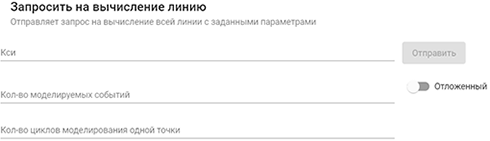
\includegraphics[width=\textwidth]{figures/request-line.png}
	\caption{Панель старта расчета линии значений}
	\label{fig:request-line}
\end{figure}

После выставления нужных пользователю параметров, необходимо нажать кнопку <<Отправить>> после чего данные отправяться на сервер и результат будет перерисован на интерфейсе приложения. Результаты вычислений будут добавлены на основной график в реальном времене, поэтому пользователю не нужно обновлять страницу с графиком.

Как только запрос был отправлен на сервер соездается \textit{websocket} соединение между \textit{web}-браузером пользователя и серверным приложением, тем самым подписывая клинта на получени денных от сервера, как только они будут готовы.

На графике кросс-секции $\sigma \times Br({Z}^{\prime} \rightarrow {W}^{+}{W}^{-})$ для ${Z}^{\prime}_{SSM}$ отриросовывается линия с новыми значениями в то время, как серверное приложение начинает параллельно для нескольких значений массы ${M}_{{Z}^{\prime}}$ моделировать столкновение протонов.

Так как в реальном столкновении протонов рождается очень большое количество различных частиц то моделирование такой задачи при помощи генератора \textit{PYTHIA} требудет значительных ресурсов центрального процессора сервера и занимает продолжительное время. Приложение созданное в рамках данной работы имеет \textit{web}-интерфейс, что позволяет сразу нескольком пользователям работать в нем и отправлять запросы на вычичления. В связи с этим вводится ограничение на количество параллельно зарпущеных процессов моделирования для каждого пользователя.

Даже самая простая задача расчета модели занимает большое время. К примеру запрос пользователя расчитать линию для всех значений ${M}_{{Z}^{\prime}}$, а в рамках данного проекта это пять тысячь точек на графике от 0 до 5000 ГэВ, и количеством генерируемых собыйтий займет 9,7 часа. 

В таком простом случае полученное значение будет подвержено значительной статистической ошибки. Чтобы убрать данную статистическую ошибку тербуются дополнительные циклы имметационного моделирования, что увеличивает затраченное время в разы. 

Под панелью для запроса вычислений распологается список ранее отправильных запросов, как показано на рисунке~\ref{fig:preferences}. Нажав на крестик <<X>> можно удалить линию на графике.

Все запросы на вычисление сохраняются для конкретного пользователя и загружаются из локального хранилища данных при обновлении страницы.

\begin{figure}[!h]
	\centering
	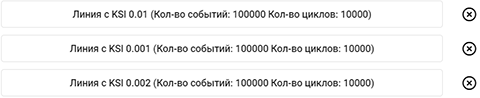
\includegraphics[width=\textwidth]{figures/preferences.png}
	\caption{Список отображаемых линий}
	\label{fig:preferences}
\end{figure}

Так как вычисления могут занять довольно много времени то вычисляются не все значения массы ${M}_{{Z}^{\prime}}$. Устанавливается шаг для вычислений к примеру 100 ГэВ и в качестве входного значения массы подставляются значения в 100 ГэВ, 200 ГэВ и т.д. Этот подход экономит значительное коливество ресурсов вычислительноый машины и экономит время для полусения общей картины поведения распределения ограничений на угол смешивания. Дополнительно на стороне сервера предусмотрено хранение уже рассчитаных результатов по выходным данным имметационного моделирования.

Как видно из рисунка~\ref{fig:offline-calc} у пользователя есть возможно отправить <<Отложенный>> запрос на вычисление для удобства вычисления линий. Отложенный запрос означает, что запрос добавиться в очередь на вычислесения на стороне сервера. Запрос будет сохраняться до того момента пока вычислительные ресурсы не осободяться и только после этого запрос обработается и начнется процесс имметационного моделирования.

\begin{figure}[!h]
	\centering
	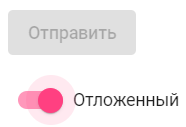
\includegraphics[width=0.4\textwidth]{figures/offline-calc.png}
	\caption{Переключатель в <<отложенный>> режим отправки запросов}
	\label{fig:offline-calc}
\end{figure}

Предусмотрена возможность отправлять запросы на вычисление только одной точки на графике. Данная возможно позволяет узнать точное значение кросс-секции $\sigma \times Br({Z}^{\prime} \rightarrow {W}^{+}{W}^{-})$ для конкретной массы ${Z}^{\prime}_{SSM}$-бозона и не тратить время на вычисления значений всех масс ${M}_{{Z}^{\prime}}$ для заданной $\xi$. Панель позволяющая отправлять такие запросы представлена на картинке~\ref{fig:request-point}.

\vspace{16pt}
\begin{figure}[!h]
	\centering
	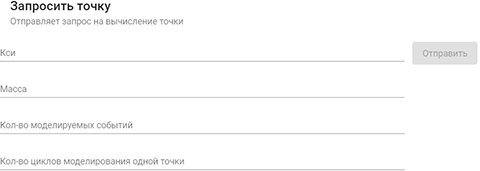
\includegraphics[width=\textwidth]{figures/request-point.png}
	\caption{Панель старта расчета одного значения}
	\label{fig:request-point}
\end{figure}

Общий процесс вычиления всех значений для масс ${M}_{{Z}^{\prime}}$ отображается в виде прогресс бара в самом низу веб страницы. Как показано на рисунке~\ref{fig:progress} данный элемент не имеет каких-либо точек взаимодействия с пользователем и несет лишь информативный характер.

\begin{figure}[!h]
	\centering
	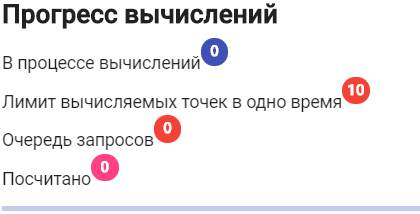
\includegraphics[width=\textwidth]{figures/progress.png}
	\caption{Прогресс вычислений}
	\label{fig:progress}
\end{figure}

Компонент <<Прогресс вычислений>> содержит комплексную информацию о ходе вычислений: количество вычисляемых значений в данный момент времени, лимит вычисляемых точек в одно время для сессии одного пользователя, очередь запросов от пользователя и количество успешно полученных результатов.

Так как вычисления могут занять довольно много времени то вычисляются только текущие запросы для текущей сессии пользователя. К примеру если, лимит на вычисления равен десять запросов в одно время и пользователь запустил процесс вычиления целой линии значений, а после закрыл старницу \textit{web}-приложения то будут произведены вычисления только этих десяти значений. Далнейшие вычисления будут возобновлены, когда пользователь внонь откроет страницу \textit{web}-интерфейса или другой пользователь отправить запрос на вычисление с теми же входными параметрами.

Интерфейс результатов и вычислений выполнен в виде \textit{SVG} элемента и состоит из графика кросс-секции $\sigma \times Br({Z}^{\prime} \rightarrow {W}^{+}{W}^{-})$ для масс ${M}_{{Z}^{\prime}}$ (рисунок~\ref{fig:graph-1}).

\begin{figure}[!h]
	\centering
	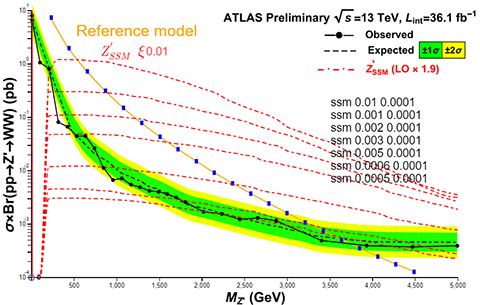
\includegraphics[width=\textwidth]{figures/graph-1.png}
	\caption{Панель старта расчета линии значений}
	\label{fig:graph-1}
\end{figure}

На графике отображены статические элементы полученные из математических формул и вычислений, а также данные не вычисляемые в рамках данной диссертации и полученные от коллаборации \textit{ATLAS}, такие  как \textit{reference model}, \textit{observed} значения, \textit{expected} значения с областью в два стандартных отклонения~\cite{2part-pankov}.

Представленный на рисунке~\ref{fig:graph-1} график имеет элемент управления - вертикальная красная линия. Данная линия добавлена, чтобы помочь пользователю определить занчание кросс-секции для массы ${M}_{{Z}^{\prime}}$ и выбранным углом смешивания $\xi$. Близлежащие значения к данной вертикальной линии будут подсвечены на графике и их точное значение всегда отображается в правой части графика.

Перейдя на вкладку <<Результат>> из меню приложения (рисунок~\ref{fig:menu}) пользователю будет предоставлен результат работы приложения, который показан на рисунке~\ref{fig:graph-result}.

Результат представляет собой график зависемости угла смешивания $\xi$ и массы ${M}_{{Z}^{\prime}}$ и отражает ограничения на угол смешивания ${Z}^{\prime}$-бозонов в модели \textit{SSM}. 

Значениями ломаной \textit{Observed} являются точки ($\xi$) пересечения моделируемых линий и кривой \textit{expected}, которые отображены на рисунке~\ref{fig:graph-1}. В данной диссертационной работе при помощи разработанной имметационной модели рождения $Z^\prime$ - бозонов в протон-протонных столкновениях с учетом эффектов $Z$ - $Z^\prime$ смешивания были получены ограничение на угол смешивания ${Z}^{\prime}$-бозонов для до светимости 3000 фб${}^{−1}$ и равняется $6*{10}^{-5}$.

\begin{figure}[!h]
	\centering
	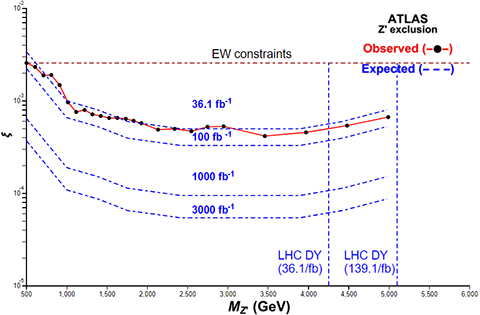
\includegraphics[width=\textwidth]{figures/graph-result.png}
	\caption{Ограничения на угол смешивания $Z$-${Z}^{\prime}$ полученные из обработки данных имитационного моделирования}
	\label{fig:graph-result}
\end{figure}

Изходя из того, что большая часть использованной литературы при исследовании проблемы описанной в данной диссертационной работе является англоязычной было принято решение реализовать возможность смены языка на котором отображается текст приложения. Такой функционал добавлен в правом верхнем углу \textit{web}-интерфейса, рисунок~\ref{fig:language-switch}.

\vspace{18pt}
\begin{figure}[!h]
	\centering
	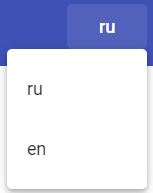
\includegraphics[width=0.3\textwidth]{figures/language-switch.png}
	\caption{Смена языка \textit{web}-страницы}
	\label{fig:language-switch}
\end{figure}


\section{Выводы}
%Данная глава посвящена имитационному моделированию процесса рождения ${Z}^{\prime}$-бозонов в протон-протнных столкновениях с учетом эффектов $Z$-${Z}^{\prime}$ смешивания в условиях эксперимента \textit{ATLAS} на Большом адронном коллайдере и разработке необходимых средств программного обеспечения.

В результате реализации предложенной математической модели процесса рождения ${Z}^{\prime}$-бозонов в протон-протнных столкновениях с последующим распадом на пару ${W}^{+}{W}^{-}$ бозонов и учета эффектов $Z$-${Z}^{\prime}$ смешивания были достигнуты следующие цели: 
\begin{enumerate}
	\item[--] реализована имитационная модель процесса рождения ${Z}^{\prime}$-бозонов в протон-протнных столкновениях с последующим распадом на пару ${W}^{+}{W}^{-}$ бозонов, отличающиюся от известных моделей учетом эффектов $Z$-${Z}^{\prime}$ смешивания;
	\item[--] реализованы необходимые программные средства для имитационного моделирования процесса
	рождения ${Z}^{\prime}$-бозонов в протон-протнных столкновениях с учетом эффектов $Z$-${Z}^{\prime}$ смешивания в условиях эксперимента \textit{ATLAS} на Большом адронном коллайдере, отличающиюся от существующих тем, что программный модуль собран в \textit{Docker} образ позволяющий быстро проводить имитационное моделирование без установки необходимых программных средств.
\end{enumerate}


\chapter{ТЕСТИРОВАНИЕ И ВЕРИФИКАЦИЯ РАЗРАБОТАННОГО ПРИЛОЖЕНИЯ}
\section{Верификация работы программы}
Для верификации вычислений приложения использовались статьи написанные по реальным экспериментальным данным полученных от коллабора-ции \textit{ATLAS}. Верифиционными данными являются ограничения на эффекты $Z$-${Z}^{\prime}$ смешивания на Большом Адронном колайдере.

Изучение процесса рождения ${W}^{+}{W}^{-}$ бозонной пары на Большом адронном коллайдере позволяет исследовать спонтанное нарушение калибровочной симметрии стандартной модели (\textit{SM}) и может использоваться для поиска новых явлений за пределами \textit{SM}. Дополнительные нейтральные векторные ${Z}^{\prime}$-бозоны, распадающиеся на заряженные калибровочные векторные пары бозонов ${W}^{+}{W}^{-}$, предсказаны во многих сценариях новой физики, включая модели с расширенным калибровочным сектором. Процесс $pp \rightarrow {W}^{+}{W}^{-}$  позволяет установить жесткие ограничения на угол смешивания $\xi$ для $Z$-${Z}^{\prime}$ и массу ${Z}^{\prime}$, ${M}_{{Z}^{\prime}}$. В настоящей работе впервые получены ограничения на параметры ${Z}^{\prime}$ смешивания в плоскости $\xi$–${M}_{{Z}^{\prime}}$, полученные из экспериментальных данных \textit{ATLAS} и \textit{CMS} на \textit{LHC} при энергии 13 ТэВ и светимостями 36,1 и 35,9 фб${}^{−1}$, соответственно. Область исключения была значительно расширена по сравнению с полученной из предыдущего анализа, выполненного с данными \textit{Tevatron}, а также с данными \textit{LHC}, собранными при 7 и 8 ТэВ. Полученные ограничения~\cite{2part-pankov} на угол смешивания $Z$-${Z}^{\prime}$ существенно превосходят ограничения, ранее полученные из глобального анализа электрослабых данных.

Многие новые физические сценарии (\textit{NP}) за пределами \textit{SM}, включая суперструнные и лево-симметричные модели, предсказывают существование новых нейтральных и заряженных калибровочных бозонов, которые могут быть достаточно легкими, чтобы быть доступными на текущих и / или будущих коллайдерах. Поиск этих новых нейтральных ${Z}^{\prime}$ и заряженных ${W}^{\prime}$ калибровочных бозонов является важным аспектом экспериментальной программы физики высокоэнергетических коллайдеров. Здесь рассматриваются  эффекты ${Z}^{\prime}$-бозонов. Существующие ограничения на прямое рождение на \textit{LHC} и виртуальные эффекты на Большом электронно-позитронном коллайдере (\textit{LEP}) путем интерференции или смешения с $Z$-бозоном подразумевают, что любой новый ${Z}^{\prime}$-бозон довольно тяжелый и очень мало смешивается с $Z$-бозоном. В зависимости от рассматриваемой теоретической модели массы ${Z}^{\prime}$ порядка 4,5 ТэВ и углы смешивания $Z$-${Z}^{\prime}$ на уровне нескольких промилле исключены. Угол смешивания сильно ограничен очень высокоточными экспериментами на \textit{LEP} и линейным коллайдером \textit{SLAC} (\textit{SLC}).

\begin{figure}[!h]
	\centering
	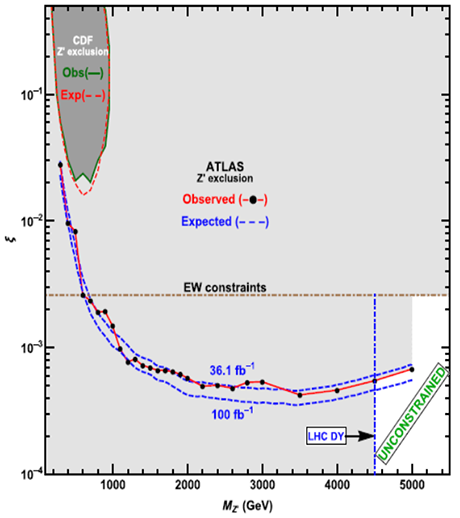
\includegraphics[width=\textwidth]{figures/verify-1.png}
	\caption{Ограничения на угол смешивания $Z$-${Z}^{\prime}$ полученные из обработки данных эксперимента \textit{ATLAS}}
	\label{fig:verify-1}
\end{figure}

\begin{figure}[!h]
	\centering
	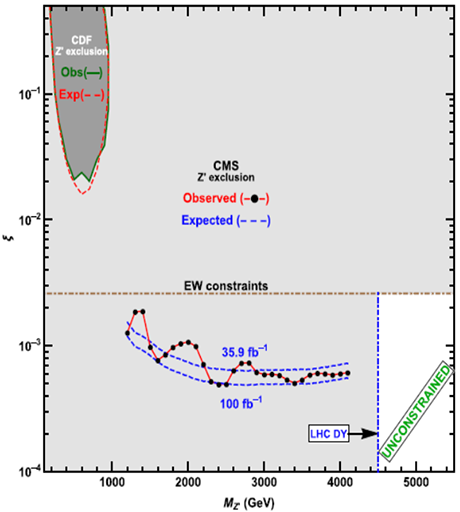
\includegraphics[width=\textwidth]{figures/verify-2.png}
	\caption{Ограничения на угол смешивания $Z$-${Z}^{\prime}$ полученные из обработки данных эксперимента \textit{CMS}}
	\label{fig:verify-2}
\end{figure}

Более подробно детали анализа данных экспериментов \textit{ATLAS} и \textit{CMS} представлены в работе~\cite{2part-pankov}. В результате обработки данных по измерению процесса рождения ${W}^{+}{W}^{-}$ пар в протон-протонных столкновениях получены экспериментальные ограничения на угол смешивания ${Z}^{\prime}$-бозонов в модели \textit{SSM}, которые составили $\xi$ < 0,0004 (рис.~\ref{fig:verify-1}, рис.~\ref{fig:verify-2}), что на порядок лучше результатов полученных ранее из глобального анализа электрослабых данных.
\section{Анализ результатов верификации}
Во время выполнения приложения могут возникать различные исключительные ситуации, которые могут пагубно сказаться на процессе работы приложения, поэтому эти ошибки необходимо предусмотреть и сделать их обработку.
\section{Вычислительный эксперимент}
В рамках диссертационной работы проводилось имитационное моделирование процесса рождения ${Z}^{\prime}$-бозонов и распад ${W}^{+}{W}^{-}$ бозонов на Большом адронном коллайдере. В ходе моделирования были получены плотность вероятности рождения ${Z}^{\prime}$-бозонов для заданных входных параметров угла смешивания $\xi$ и массы бозона ${M}_{{Z}^{\prime}}$ с последующим распадом на пару ${W}^{+}{W}^{-}$ бозонов.

В ходе проведения вычислительных экспериментов было выявлено, что для получения дифференциального сечения (плотности вероятности) рождения ${Z}^{\prime}$-бозонов с точностью 95\% и выше необходимо было для каждой пары входных параметров угла смешивания $\xi$ и массы бозона ${M}_{{Z}^{\prime}}$ провести генерацию не меньше 100 000 событий столкновений протонов в процессе $pp \rightarrow W^+W^- + X$. 

Из-за присутствия статистической ошибки генератора даже при таком большом количестве генерируемых событий заданная точность не достигалась. Для уменьшения статистической ошибки проводились дополнительные итерации имитационного моделирования с постоянными значениями параметров угла смешивания $\xi$ и массы бозона ${M}_{{Z}^{\prime}}$, и разными значениями рандомизации для каждого цикла. Заданная точность достигалась при 10 000 циклов вычислительного эксперимента для одной точки на графике плотности вероятности рождения ${Z}^{\prime}$-бозонов.

В ходе моделирования было расчитанно 400 точек на плоскости параметров ($\sigma \times Br({Z}^{\prime} \rightarrow {W}^{+}{W}^{-})$ на ${M}_{{Z}^{\prime}}$) и смоделированно 400 миллиардов процессов столкновения протонов $pp \rightarrow W^+W^- + X$.
\section{Выводы}
С использованием разработанного программного комплекса проведено исследование процесса рождения ${Z}^{\prime}$-бозонов и последующего распад ${W}^{+}{W}^{-}$ бозонов на Большом адронном коллайдере и были получены оценки ограничений на углы смешивания ${Z}^{\prime}$-бозонов в
процессе рождения ${W}^{+}$${W}^{-}$ пар в протон-протонных столкновениях
в условиях экспериментов на Большом адронном коллайдере.Для интегральной светимости 1000 фб${}^{-1}$ и 3000 фб${}^{-1}$, которые составили  ${10}^{-4}$ и $6\times{10}^{-5}$, соответственно. Полученные оценки ограничений существенно превышают существующие экспериментальные ограничения.

Кроме этого была проведена верификация полученных результатов с
работой~\cite{2part-pankov}. Все полученные результаты успешно верифицировались,
следовательно, разработанная имитационная модель в программном комплексе
ведет себя корректно.

\newpage
\chapter*{ЗАКЛЮЧЕНИЕ}
\addcontentsline{toc}{chapter}{ЗАКЛЮЧЕНИЕ} % in Content
Целью реферата было исследование преимуществ и недостатков ОС \textit{Linux}. Был поставлен ряд задач, которые необходимо было выполнить, для достижения намеченной цели. Если рассмотреть последовательно каждый пункт, то можно сделать вывод, что цель реферата достигнута: дан развернутый ответ на вопрос, что такое \textit{Linux}. Рассмотрена поэтапно история создания ОС \textit{Linux}. Проанализированы сильные и слабые строны современных ОС, а также выявлены основные преимущества и недостатки. Сделаны соответствующие выводы о перспективе развития \textit{Linux}.

Во второй главе реферата рассмотрен процесс рождения $Z^\prime$ бозонов в протон-протонных столкновениях с учётом эффектов $Z$-$Z^\prime$ смешивания. Рассмотрены интурменты библиотеки \textit{PYTHIA} для имитационного моделирования процессов взаимодействия элементарных частиц при высоких энергиях. Исследован процесс рождения $Z^\prime$-бозонов в процессе $pp \rightarrow Z^\prime \rightarrow l^+l^- + X$ с учетом эффектов $Z$--$Z^\prime$ смешивания.

\newpage
\addcontentsline{toc}{chapter}{БИБЛИОГРАФИЧЕСКИЙ СПИСОК}
\begin{thebibliography}{9999.}


\bibitem{review-pythia}
	Леонтьев, В. В. 
	Информационные методы в физике высоких энергий 
	/ В. В. Леонтьев, И. И. Белотелов 
	— Москва : «Университетская книга», 2011.
% http://lib.sinp.msu.ru/static/tutorials/141_Leontiev_Zadahi_2011.pdf

\bibitem{review-powheg}
	Alioli, S. NLO and parton showers: the POWHEG-BOX
	/ Simone Alioli 
	// DESY, Platanenallee 6, 15738 Zeuthen, Germany – 2013. – Vol. 40. – P. 12.
% https://indico.desy.de/indico/event/1964/session/16/contribution/238/material/0/0.pdf

\bibitem{review-sherpa}
	Event generation with SHERPA
	/ Gleisberg, T. [et al.]  
	// Phys. Rev. D. – 2014. – Vol. 60. – P. 3.
% https://arxiv.org/format/0811.4622

% Java book
\bibitem{java}
	Java: the complete reference. 
	/ Schildt H. 
	// McGraw-Hill Education Group, 2016. – P. 820.
% Spring book
\bibitem{spring}
	Aspectj in action: enterprise AOP with spring applications
	/ Laddad R. 
	// Manning Publications Co., 2014. – P. 254.
% Docker book
\bibitem{docker}
	Docker in action
	/ Nickoloff J.
	// Manning Publications Co., 2016. – P. 304.
% AWS Book https://aws.amazon.com/ru/what-is-aws/#most-functionality
\bibitem{aws}
	Amazon web services in action
	/ Wittig A.
	// Manning Publications Co., 2015. – P. 500.

\bibitem{2part-1}
	За пределами Стандартной модели
	[Электронный ресурс].
	 — Режим доступа: https://elementy.ru/LHC/HEP/SM/beyondSM 
	 — Да­та доступа: 11.12.2017.


\bibitem{Krasnikov:2004}
	Н. В. Красников, В. А. 
	Матвеев. Поиск новой физики на LHC
	[Электронный ресурс].
	 — Режим доступа: http://nuclphys.sinp.msu.ru/ATLAS\_exp/at03.htm 
	 — Дата доступа: 11.12.2017.
	 
\bibitem{2part-pythia-all}
	 Official documentation
	 [Электронный ресурс].
	 — Режим доступа: http://home.thep.lu.se/~torbjorn/Pythia.html 
	 — Дата доступа: 11.12.2017.
% Статья
\bibitem{Bobovnikov:2016}
	Бобовников, И.Д. Эффекты $Z-Z^\prime$-смешивания в процессах рождения пары $W^±$-бозонов на адронных и лептонных коллайдерах высоких энергий
	/ И.Д. Бобовников, А.А. Панков.
	— Письма в ЭЧАЯ, 2016. T. 13, №1(199). С.8-35
	
\bibitem{nuclphys:weak}
	Слабое взаимодействие 
	[Электронныйресурс].
	— Режим доступа: http://nuclphys.sinp.msu.ru/enc/e149.htm
	— Дата доступа: 11.12.2017.

% Book
	 
\bibitem{2part-pankov}
	Osland, P. Probing $Z-Z^\prime$ mixing with ATLAS and CMS resonant diboson production data at the LHC at $\sqrt{s}=13$ TeV
	/ P. Osland, A.A. Pankov, A.V. Tsytrinov 
	// Physical Review D. – 2017. – Vol. 96. – P. 055040.
% 7
\bibitem{andreev-pankov:2012}
	Andreev, V. V. Constraints on the $Z-Z^\prime$ mmixing angle from data measured for the process $e^+e^- \rightarrow W^+W^-$ at the LEP2 collider
	/ V.V. Andreev, A.A. Pankov
	// Phys. At. Nucl. – 2012. – Vol. 75. – P. 76.
% 8	
\bibitem{schael:2006}
	ALEPH and DELPHI and L3 and OPAL and SLD Collaborations and LEP Electroweak Working Group and SLD Electroweak Group and SLD Heavy Flavour Group
	/ Schael, S. [et al.] 
	// Precision electroweak measurements on the Zresonance, Phys. Rep. 2006. – P. 427.
% 19
\bibitem{sirunyan:2017}
	Search for massive resonances decaying into $WW$, $WZ$ or $ZZ$ bosons in proton-proton collisions at $\sqrt{s}=13$ TeV
	/ Sirunyan, A. M. [et al.] 
	// J. High Energy Phys. – 2017. – Vol. 162. – P. 56.
% 26
\bibitem{ada-wwz:2013}
	Measurement of $W^+W^-$−production in pp collisions at $\sqrt{s}=7$ TeV with the ATLAS detector and limits on anomalous $WWZ$ and $WW_y$ couplings
	/ Ada, G. [et al.] 
	// Phys. Rev. D. – 2013. – Vol. 88. – P. 29.
% 25	
\bibitem{ada-lvlv:2013}
	Search for new phenomena in the $WW \rightarrow lvl^{\prime}v^{\prime}$ final state in $pp$ collisions at $\sqrt{s}=7$ TeV with the ATLAS detector
	/ Ada, G. [et al.] 
	// Physics Letters B. – 2013. – Vol. 3. – P. 878.
	





\end{thebibliography}

\textbf{Список публикаций соискателя}\\

1-A. Бурим~И.~П., Моделирование рождения $Z^\prime$ - бозонов в протон-протонных столкновениях с учетом эффектов $Z$ - $Z^\prime$ смешивания / Бурим~И.~П., Цитринов~А.~В., Курочка~К.~С. // V Международная конференция <<Инновации в современной науке>> -- Киев, 2019. (направлено в печать)

%1-A. Бурим~И.~П., Моделирование рождения $Z^\prime$ - бозонов в протон-протонных столкновениях с учетом эффектов $Z$ - $Z^\prime$ смешивания / Бурим~И.~П., Цитринов~А.~В., Курочка~К.~С. // Научный журнал «Доклады БГУИР». – Минск: БГУИР, 2018. (направлено в печать)

\newpage
\chapter*{ПРИЛОЖЕНИЕ А}
\addcontentsline{toc}{chapter}{ПРИЛОЖЕНИЕ А} % in Content
ыыыыыыыыыыыы

\end{document}

%%%%\bibliographystyle{gost780u}
%%%%\bibliography{liter,Liter_book,Liter_article,Liter_PHDTHESIS,Liter_preprint,Liter_conference}
%%%%\end{document}
